\subsection*{New Phytologist Supporting Information Figs S1-S18 and Tables S1-S6\\
Article title: Interaction between ploidy, breeding system, and lineage diversification\\
Authors: Rosana Zenil-Ferguson, J. Gordon Burleigh, William A. Freyman, Boris Igi\'c, Itay Mayrose and Emma E. Goldberg\\
Article acceptance date: 14 August 2019}

% check values of delta and rho D/P+A/B with(out) delta
% i.e. parameter values in figure S1 & S4 vs Table S2
\begin{suppfigure}
%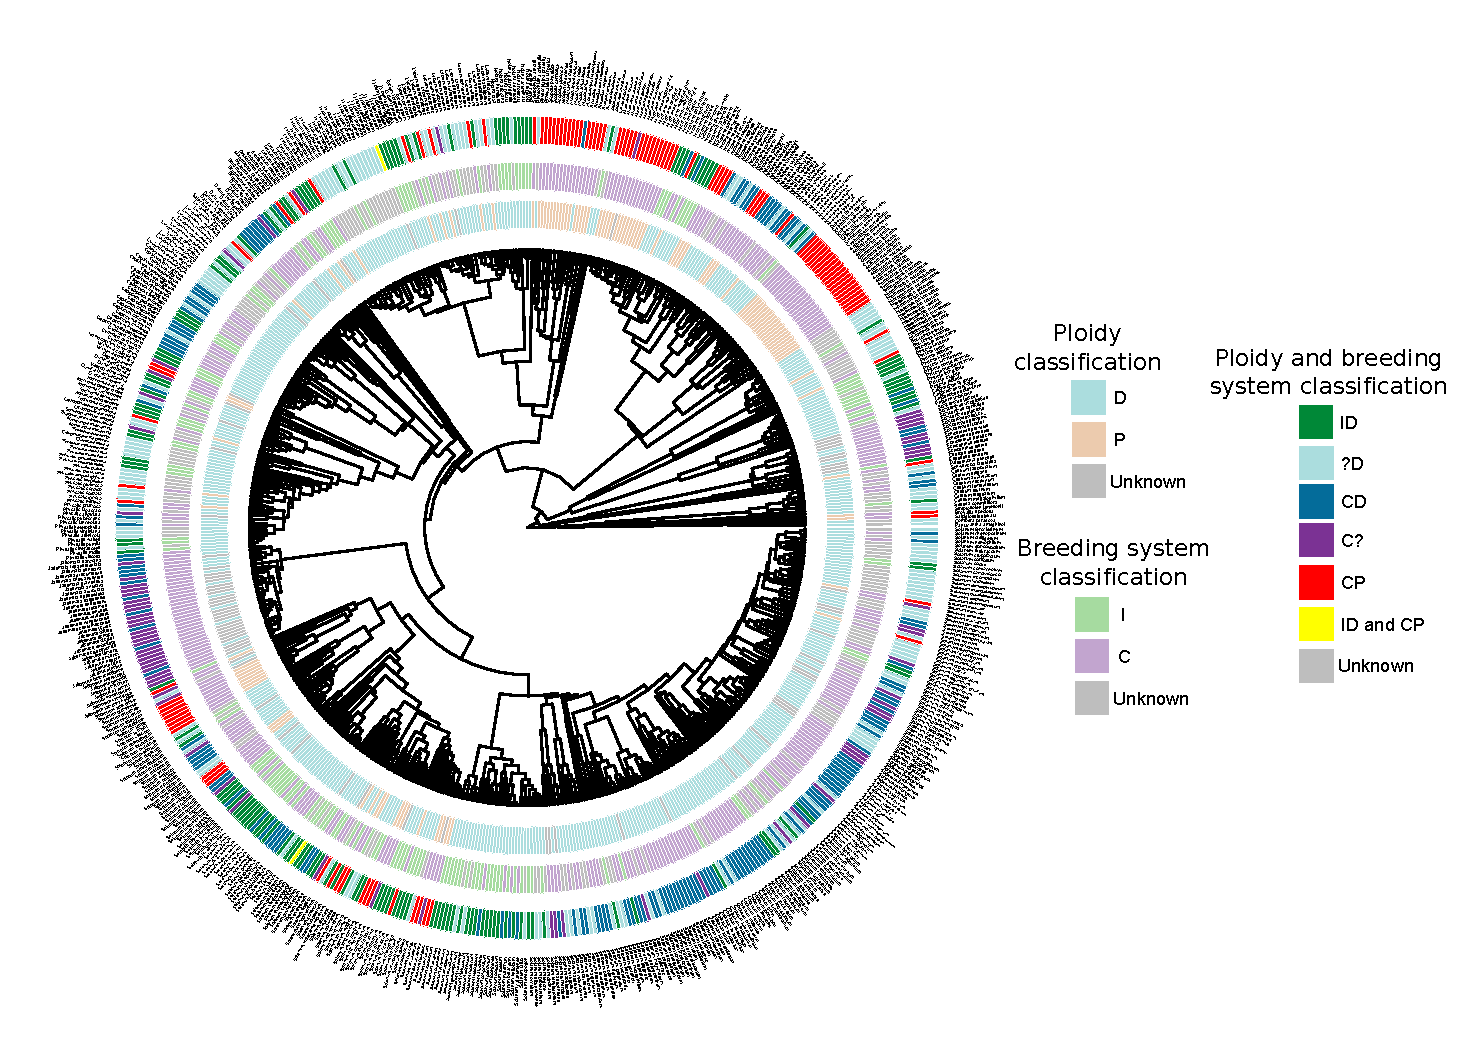
\includegraphics[width=\textwidth]{figS1.pdf}
    \caption{Ploidy and breeding system data according to three different classifications. For ploidy only models, classifications with states $D$ and $P$ were used (inner circle). For breeding system models classifications with states $I$ and $C$ were used (middle circle). For ploidy and breeding system models classifications using $ID, CD, CP$ were used (outer circle). Data with missing information in one of the traits was classified simultaneously as two possible states, for example, diploids without breeding system $?D$ were classified as $(CD, CP)$).}
    \label{fig:allmodels}
\end{suppfigure}





\begin{suppfigure} %figS2 all models
    \caption{ Twenty-nine models of diversification are proposed for the study of ploidy, breeding systems, and hidden states linked to the process of diversification. We divide the models by the type of focal trait studied (ploidy only, breeding system only, or ploidy and breeding system). The contributions of the focal trait to the diversification process can be measured by comparing the models in each of the columns. That is, the focal trait only models assume that speciation and extinction rates are only linked to the trait itself, the hidden trait only models assume that the diversification rates are  linked to unknown factors but not the trait of interest, and the focal trait with hidden trait models assume that both the focal trait and unknown factors are contributing to diversification.}
    \label{fig:allmodels}
\end{suppfigure}



\begin{suppfigure}
%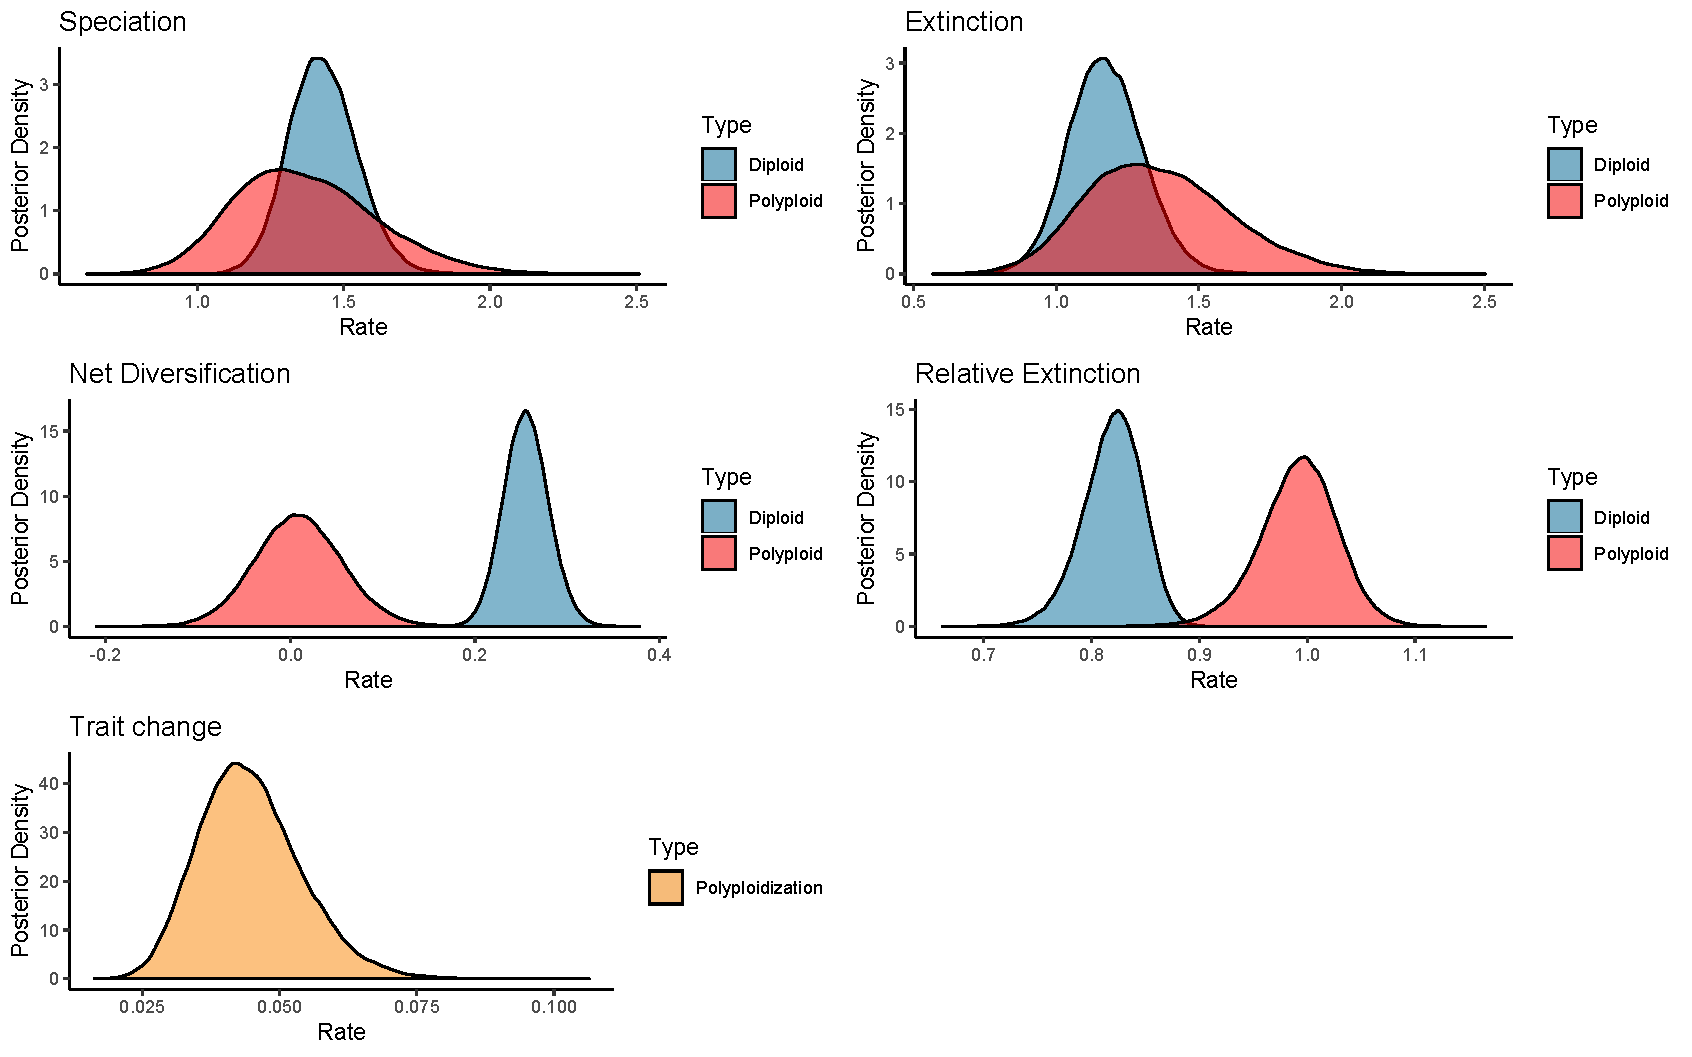
\includegraphics[width=\textwidth]{figS3.pdf}
\caption{Posterior distributions for each of the parameters in the ploidy only model (M1). Red color represents diploid state $D$ and blue color represents polyploid state $P$.  (A)Speciation rates. (B) Extinction rates. (C) Net diversification rates (speciation minus extinction from panels A and B). (D) Relative extinction rates (extinction divided by speciation from panels A and B). (E) Polyploidization rate ($\rho$).} % XXX
\label{suppfigure:DPnodip}
\end{suppfigure}

\begin{suppfigure}
%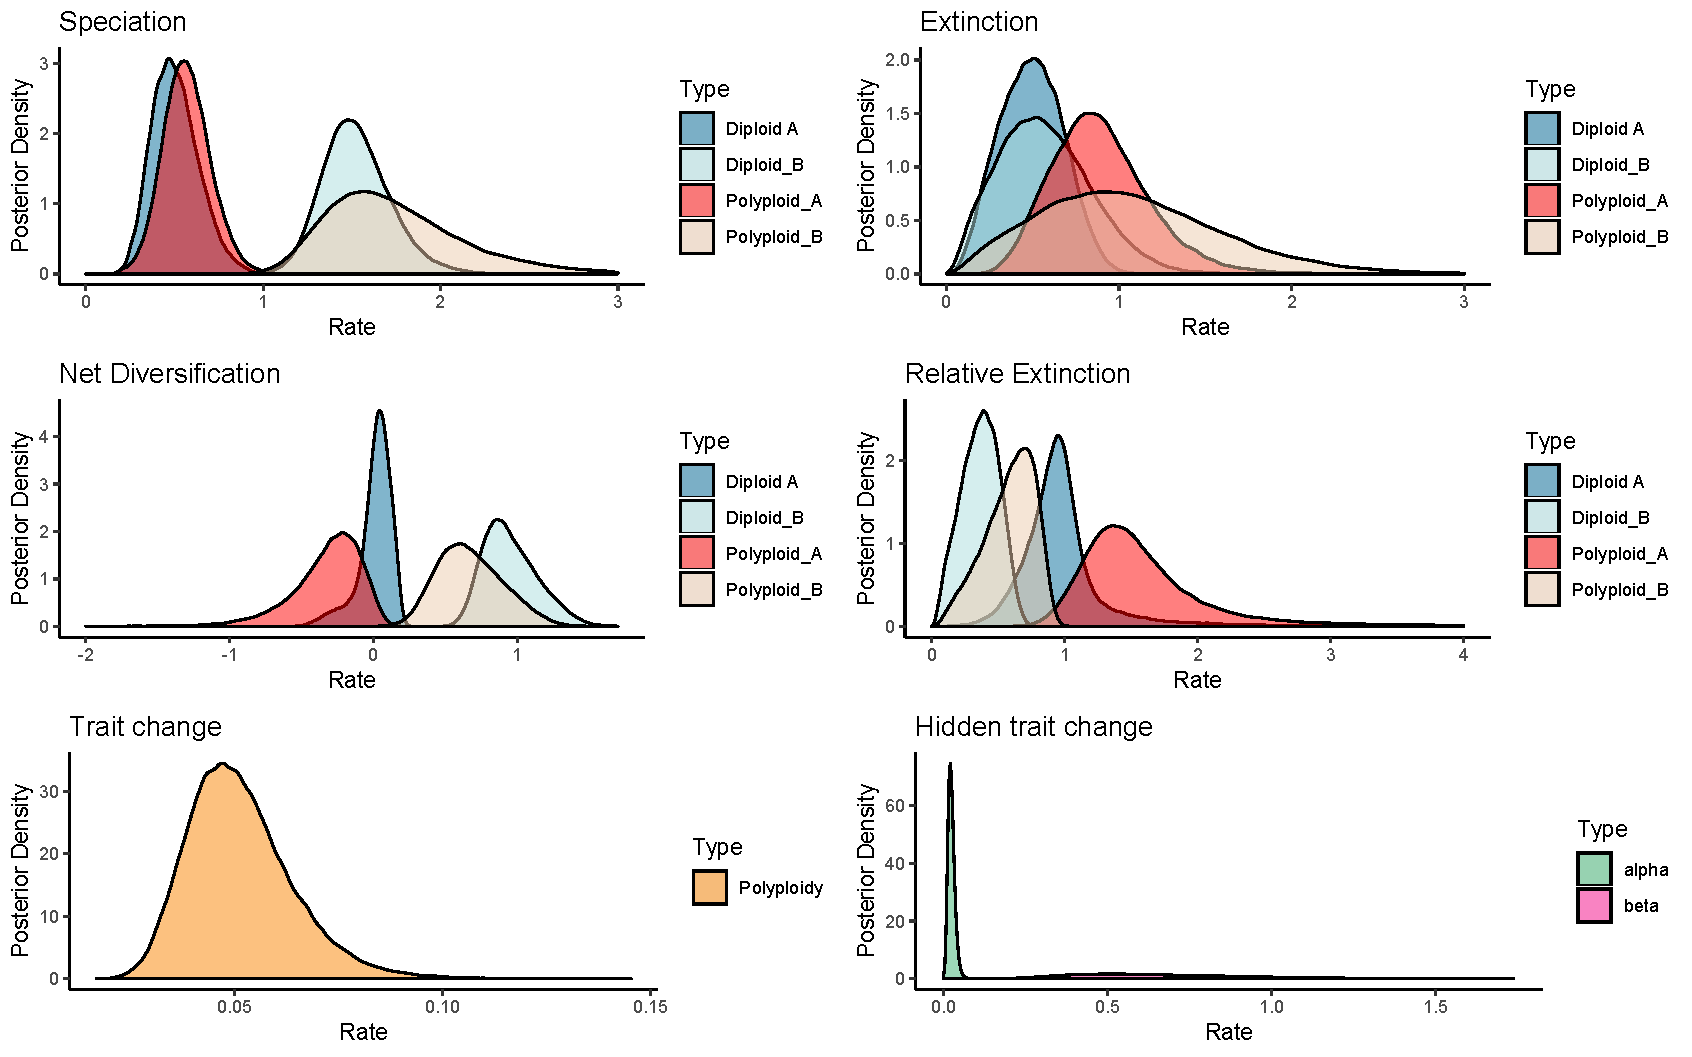
\includegraphics[width=\textwidth]{figS4.pdf}
\caption{Posterior distributions for each of the parameters in the ploidy and hidden trait model (M4). Red color represents diploid state $D$ and blue color represents polyploid state $P$. Dark colors represent hidden state $A$ and light colors hidden state $B$.  (A) Speciation rates. (B) Extinction rates. (C) Net diversification rates (speciation minus extinction from panels A and B). (D) Relative extinction rates (extinction divided by speciation from panels A and B). (E) Polyploidization rate ($\rho$). (F) Transition rates between hidden states ( $\alpha$ and $\beta$).} % XXX
\label{suppfigure:DPnodipAB}
\end{suppfigure}

\begin{suppfigure}
%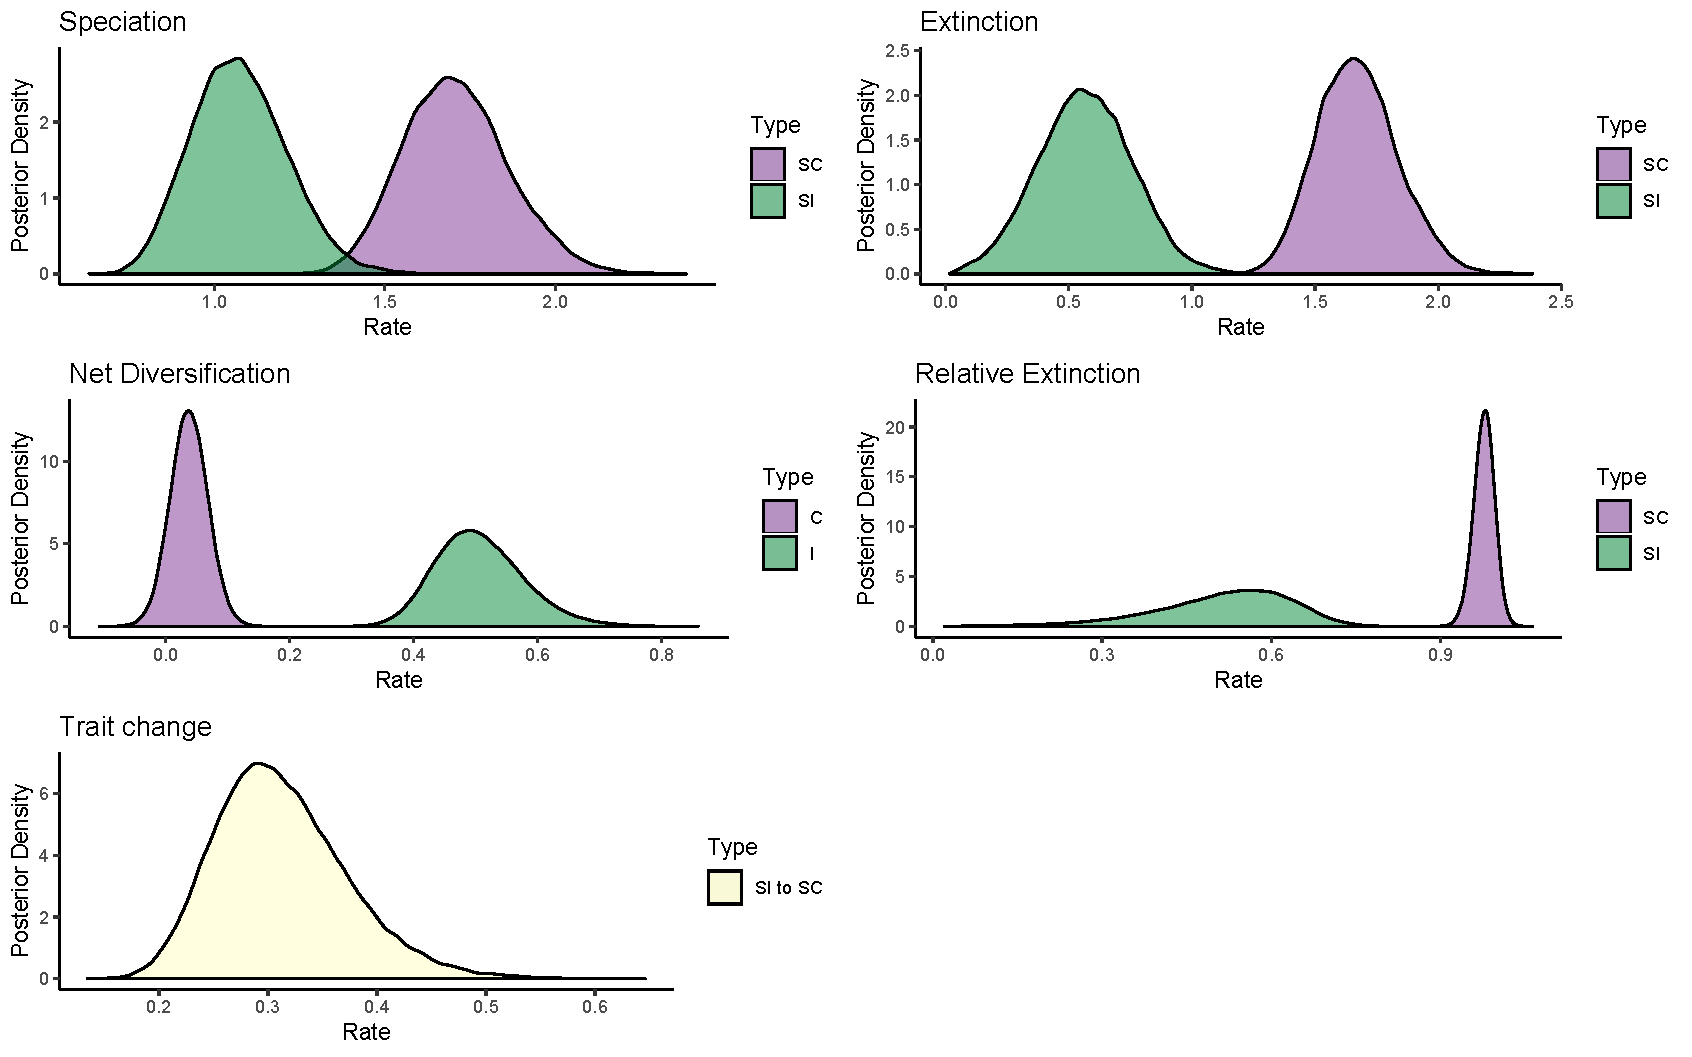
\includegraphics[width=\textwidth]{figS5.pdf}
\caption{Posterior distributions for each of the parameters in the breeding system only model (M11). Green color represents self-incompatible state $I$ and purple color represents self-compatible state $C$.  (A) Speciation rates. (B) Extinction rates. (C) Net diversification rates (speciation minus extinction from panels A and B). (D) Relative extinction rates (extinction divided by speciation from panels A and B). (E) Self-incompatible to self-compatible transition rate ($q_IC$).} % XXX
\label{suppfigure:IC}
\end{suppfigure}


\begin{suppfigure}
%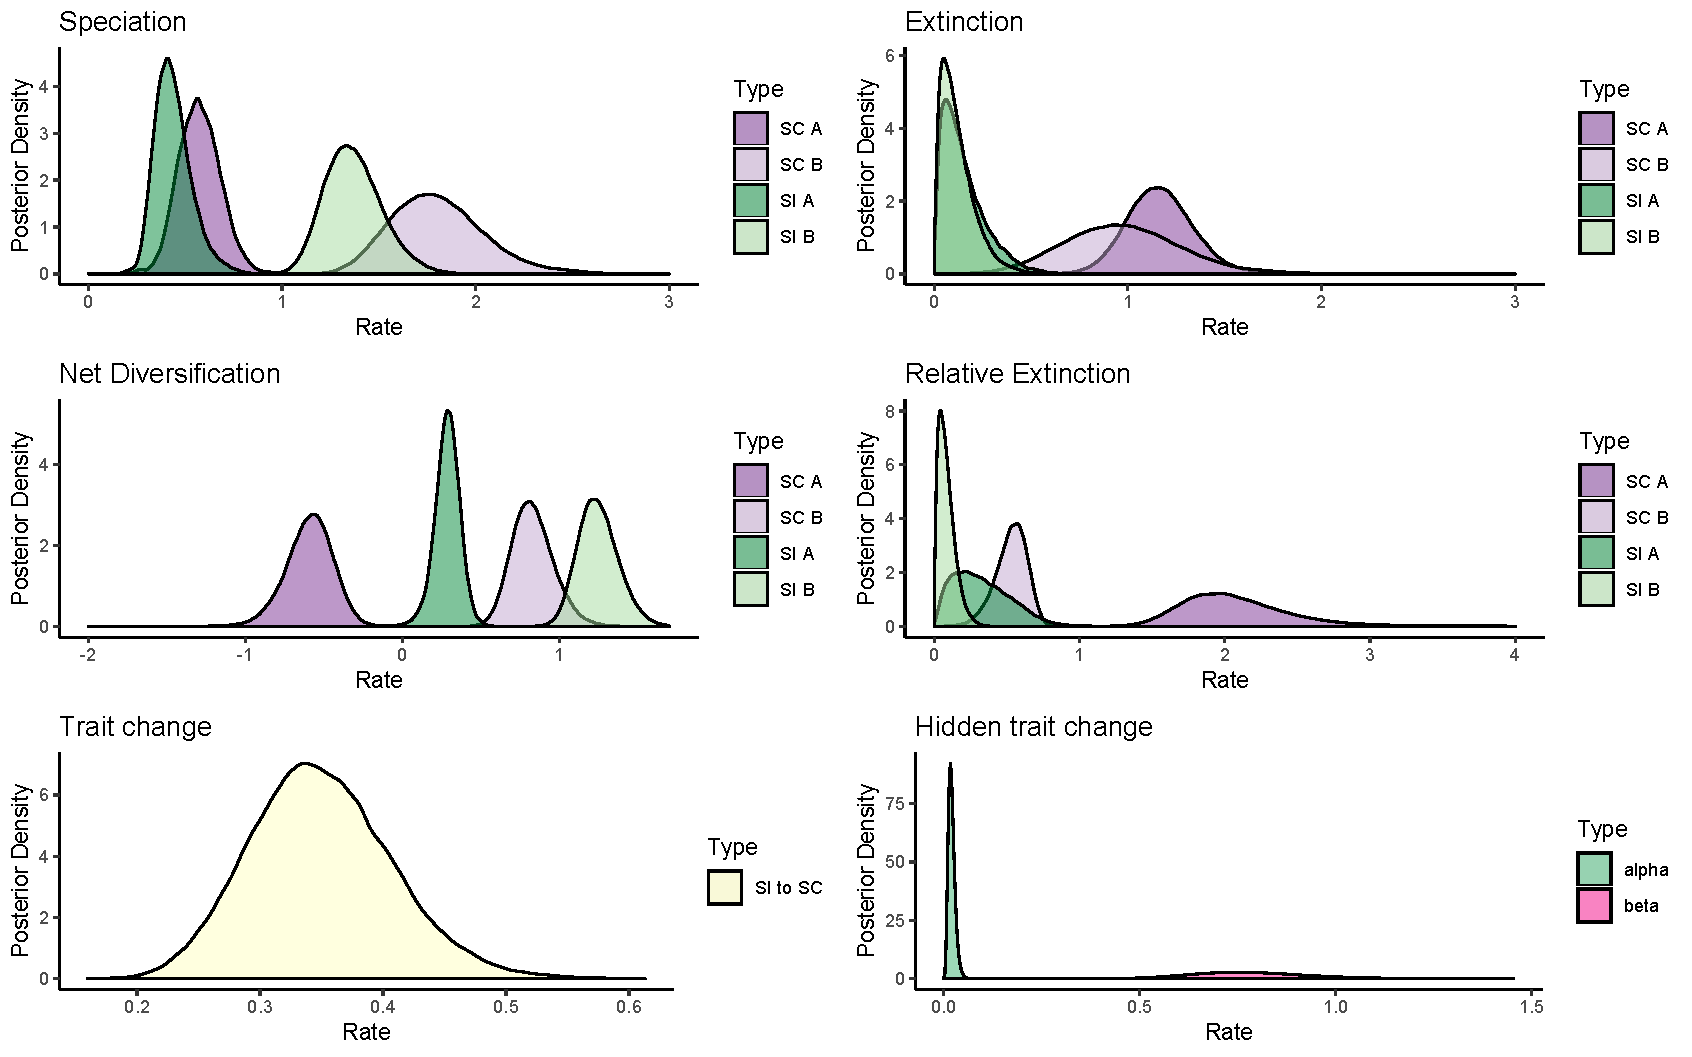
\includegraphics[width=\textwidth]{figS6.pdf}
\caption{Posterior distributions for each of the parameters in the breeding system and hidden trait model (M14). Green color represents self-incompatible state $I$ and purple color represents self-compatible state $A$. Dark colors represent hidden state $A$ and light colors hidden state $B$.  (A) Speciation rates. (B) Extinction rates. (C) Net diversification rates (speciation minus extinction from panels A and B). (D) Relative extinction rates (extinction divided by speciation from panels A and B). (E) Self-incompatible to self-compatible transition rate ($q_IC$). (F) Transition rates between hidden states ( $\alpha$ and $\beta$).} % XXX
\label{suppfigure:ICAB}
\end{suppfigure}


\begin{suppfigure}
%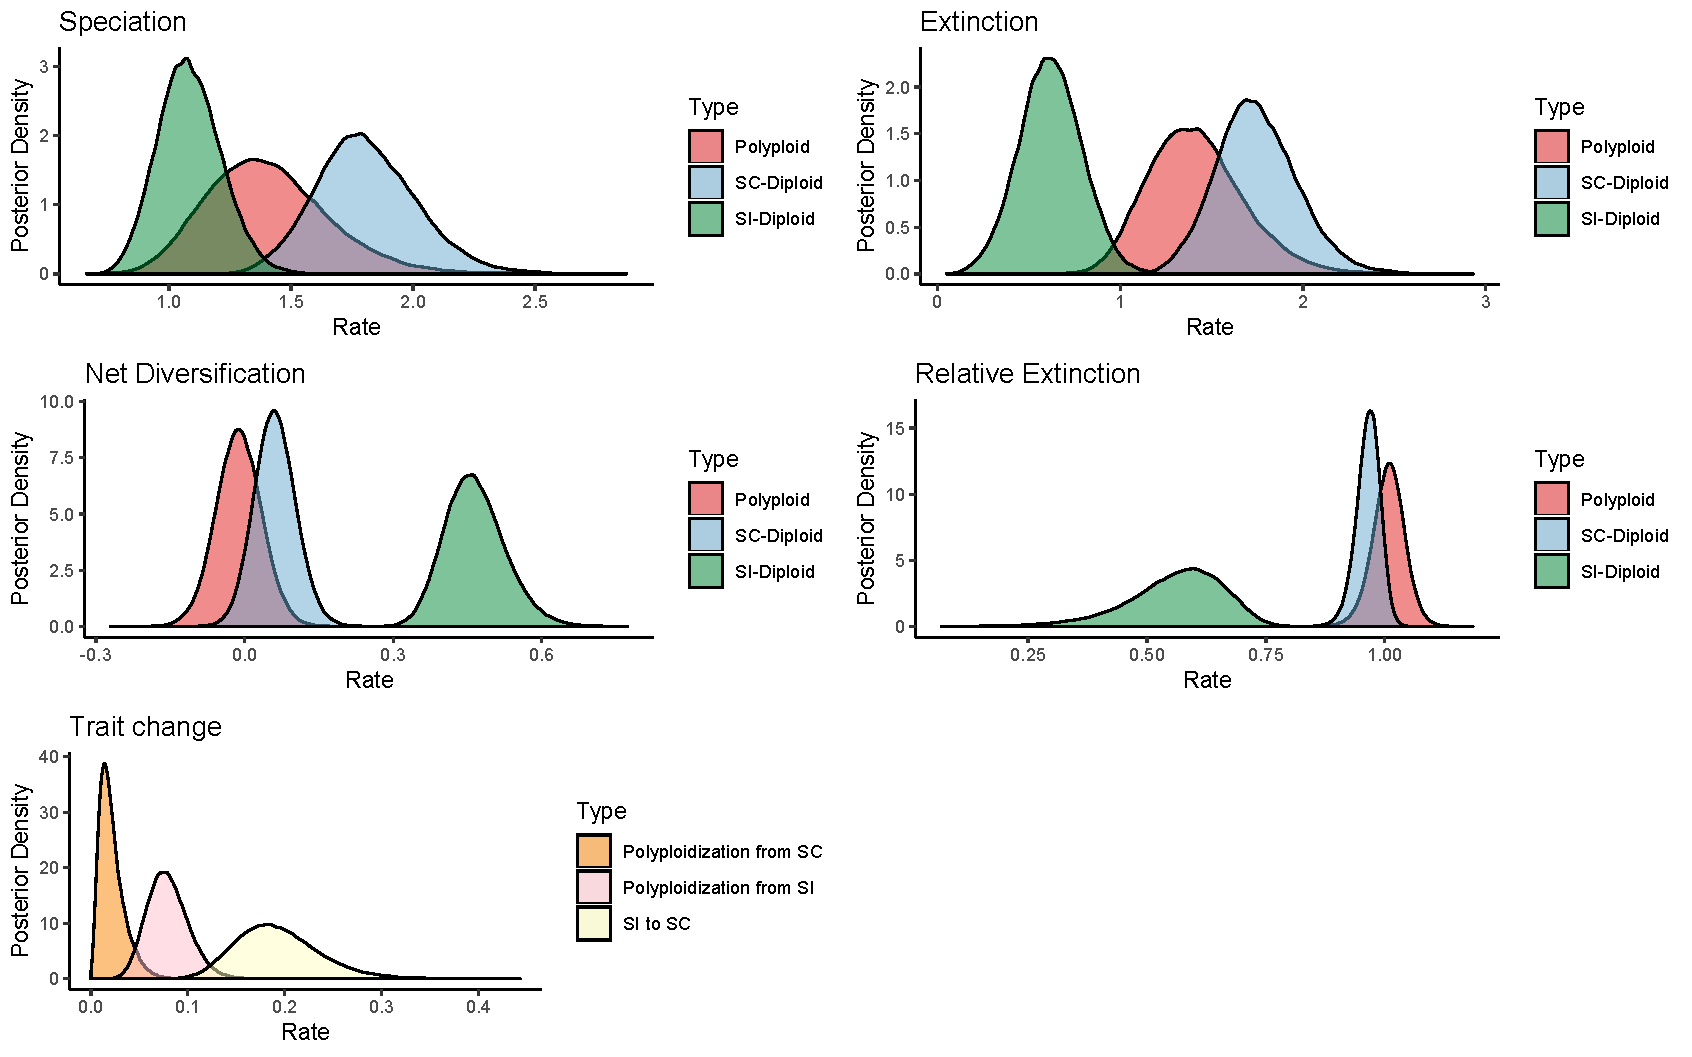
\includegraphics[width=\textwidth]{figS7.pdf}
\caption{Posterior distribution for each of the parameters in the ploidy and breeding system model (M16). Green color represents self-incompatible diploid state $ID$, blue color is the self-compatible and diploid state $CD$ and pink represents self-compatible polyploid state $CP$.  (A) Speciation rates. (B) Extinction rates. (C) Net diversification rates (speciation minus extinction from panels A and B). (D) Relative extinction rates (extinction divided by speciation from panels A and B). (E) Self-incompatible to self-compatible transition rate ($q_IC$, yellow), polyploidization rate from self-incompatible ($\rho_I,$ light pink), and polyploidization from self-compatible ($\rho_c$, orange).} % XXX
\label{suppfigure:IDCDCPnodip}
\end{suppfigure}

\begin{suppfigure}
%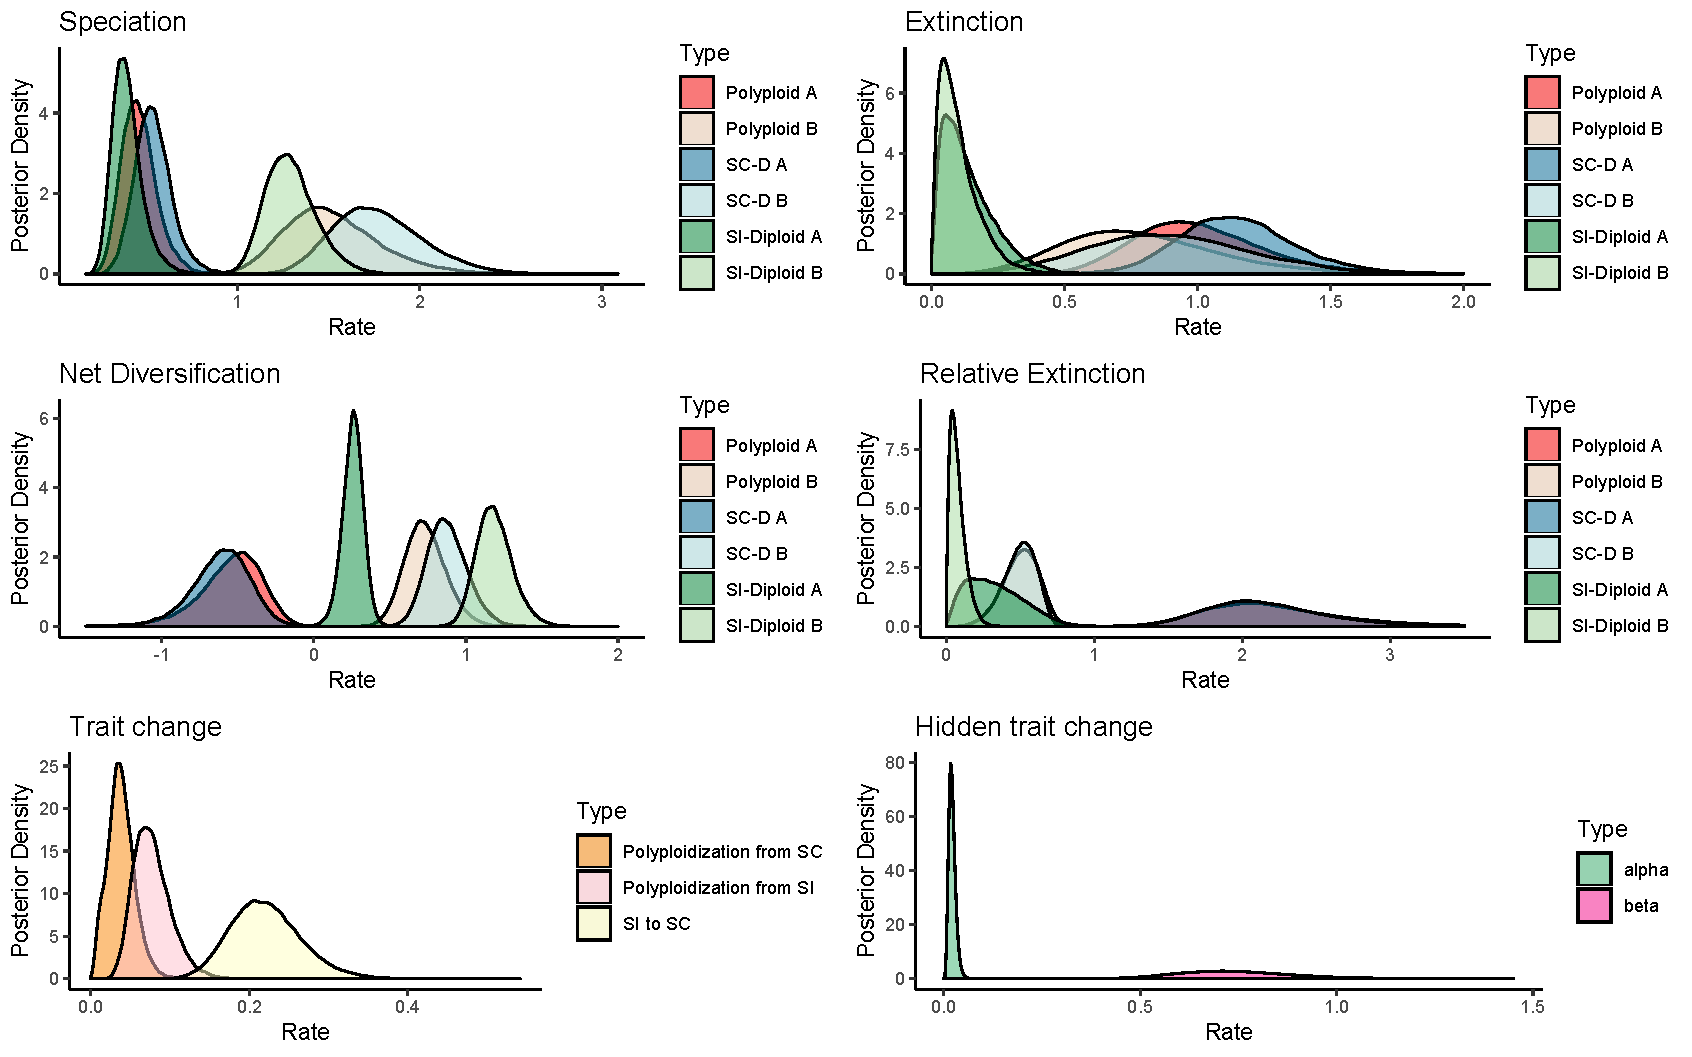
\includegraphics[width=\textwidth]{figS8.pdf}
\caption{Posterior distribution for each of the parameters in the ploidy, breeding system, and hidden trait model (M19). Green color represents self-incompatible diploid state $ID$, blue color is the self-compatible and diploid state $CD$ and pink represents self-compatible polyploid state $CP$. Dark colors represent hidden state $A$ and light colors hidden state $B$.  (A) Speciation rates. (B) Extinction rates. (C) Net diversification rates (speciation minus extinction from panels A and B). (D) Relative extinction rates (extinction divided by speciation from panels A and B). (E) Self-incompatible to self-compatible transition rate ($q_IC$, yellow), polyploidization rate from self-incompatible ($\rho_I,$ light pink), and polyploidization from self-compatible ($\rho_c$, orange). (F) Transition rates between hidden states ( $\alpha$ and $\beta$).}% XXX
\label{suppfigure:IDCDCPnodipAB}
\end{suppfigure}

\begin{suppfigure}
%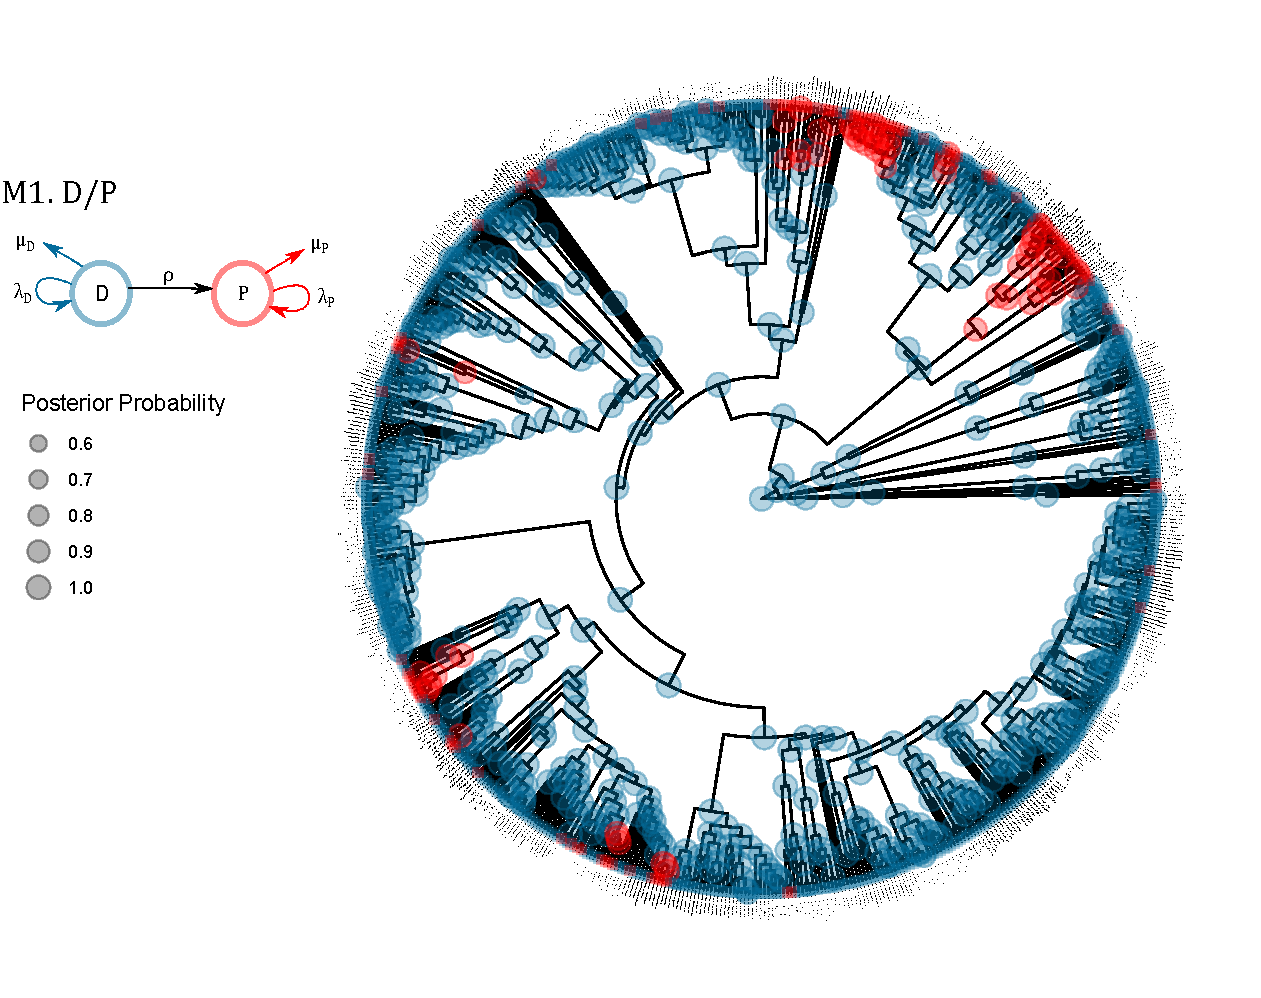
\includegraphics[width=\textwidth]{figS9.pdf}
\caption{Ancestral state estimation showing the maximum \emph{a posteriori} estimates of the marginal probability distributions for each of the 650 internal nodes under  the ploidy only model (M1). } % XXX
\label{suppfigure:DPnodipasr}
\end{suppfigure}



\begin{suppfigure}
%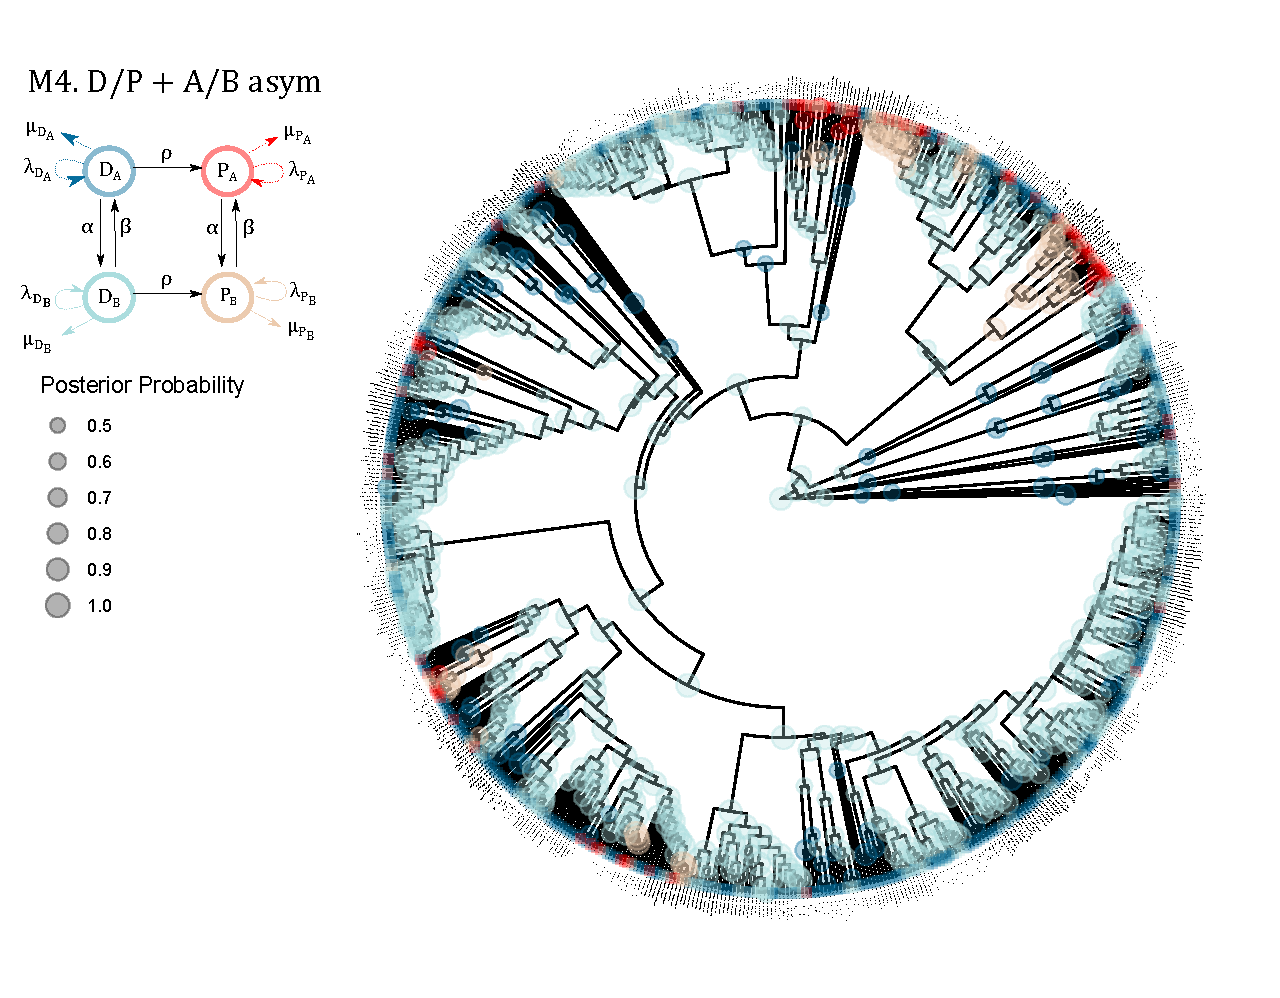
\includegraphics[width=\textwidth]{figS10.pdf}
\caption{Ancestral state estimation showing the maximum \emph{a posteriori} estimates of the marginal probability distributions for each of the 650 internal nodes under the ploidy and hidden states model (M4).} % XXX
\label{suppfigure:DPnodipABasr}
\end{suppfigure}


\begin{suppfigure}
%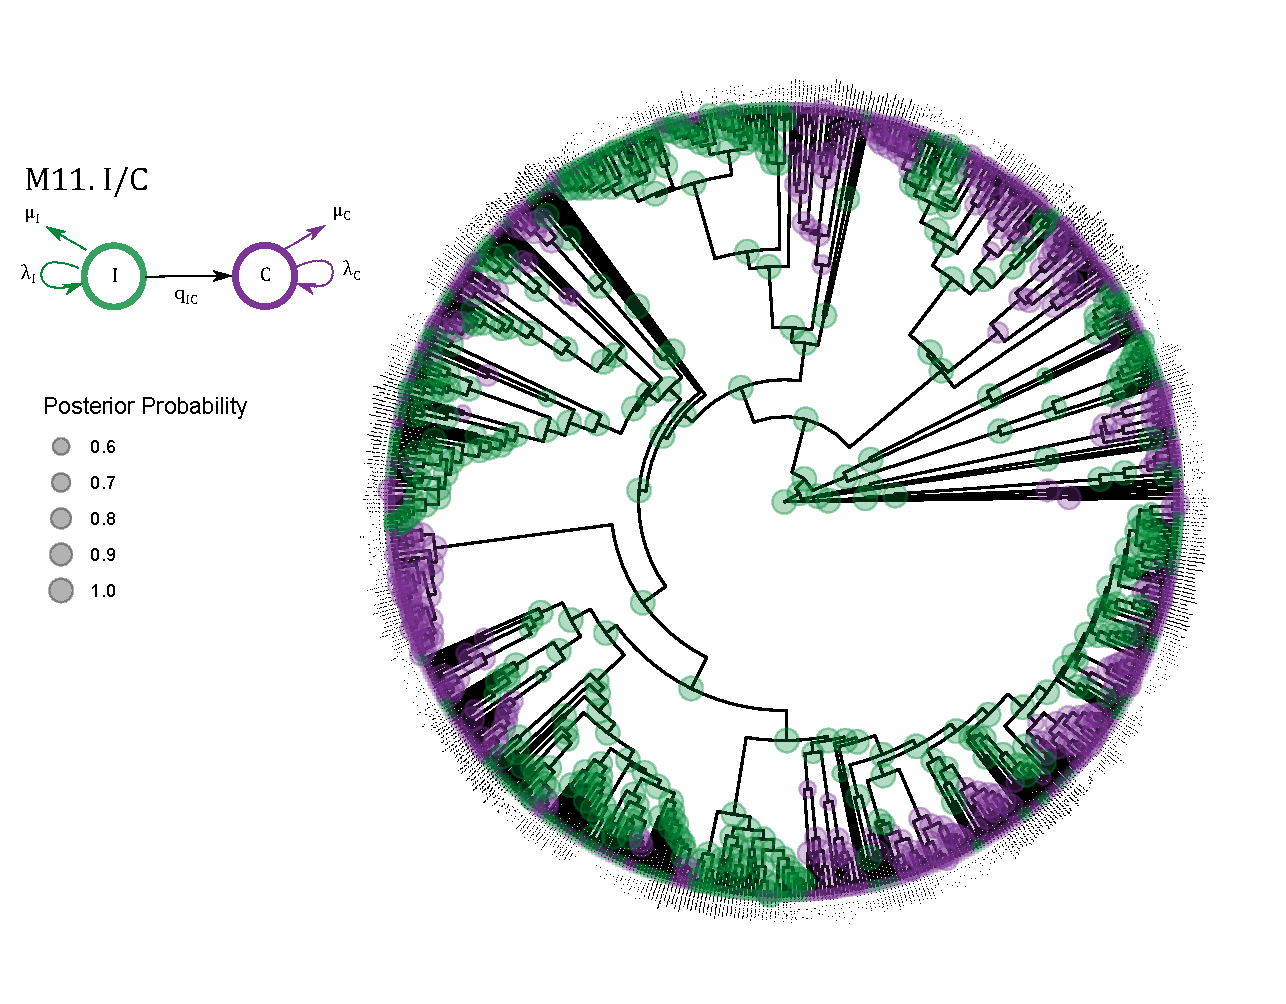
\includegraphics[width=\textwidth]{figS11.pdf}
\caption{Ancestral state estimation showing the maximum \emph{a posteriori} estimates of the marginal probability distributions for each of the 650 internal nodes under the  breeding system only model (M11).} % XXX
\label{suppfigure:ICasr}
\end{suppfigure}



\begin{suppfigure}
%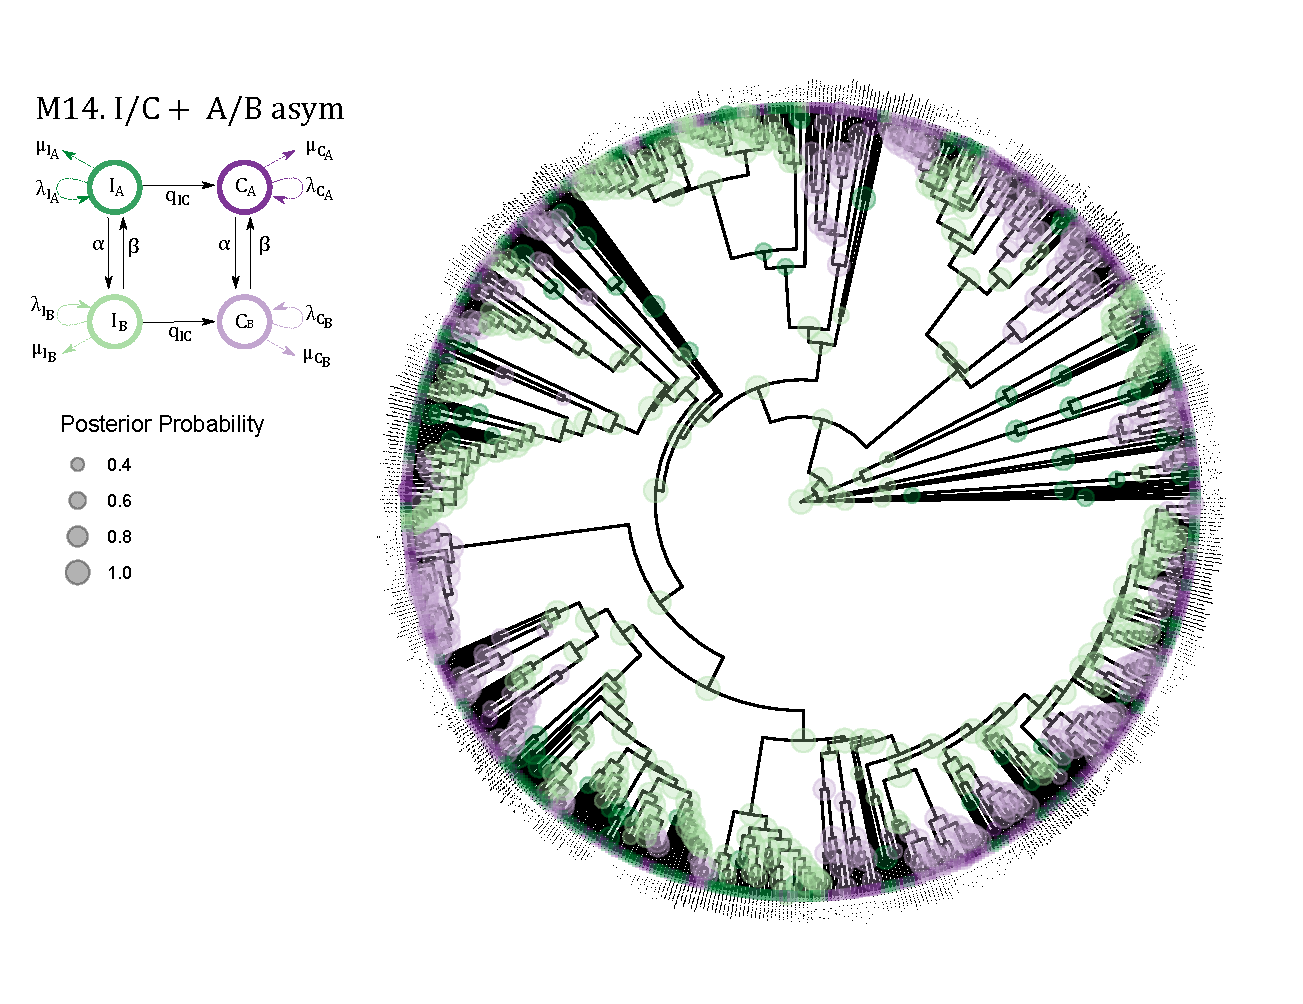
\includegraphics[width=\textwidth]{figS12.pdf}
\caption{Ancestral state estimation showing the maximum \emph{a posteriori} estimates of the marginal probability distributions for each of the 650 internal nodes under the breeding system and hidden states model (M14.} % XXX
\label{suppfigure:ICABasr}
\end{suppfigure}


\begin{suppfigure}
%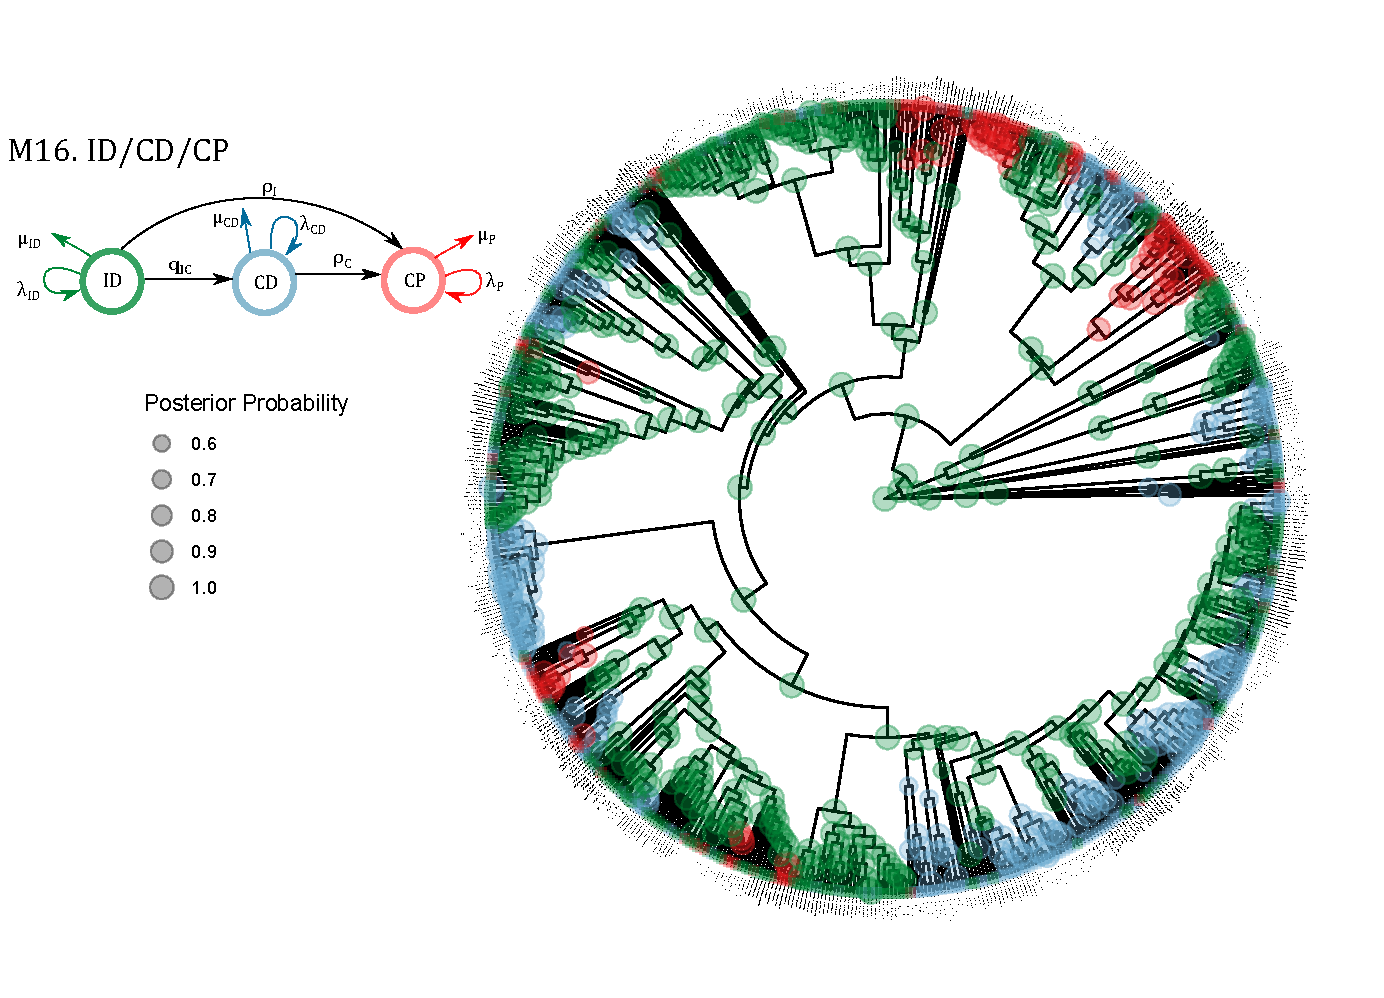
\includegraphics[width=\textwidth]{figS13.pdf}
\caption{Ancestral state estimation showing the maximum \emph{a posteriori} estimates of the marginal probability distributions for each of the 650 internal nodes under the ploidy and breeding system model (M16).} % XXX
\label{suppfigure:IDCDCPnodipasr}
\end{suppfigure}



\begin{suppfigure}
%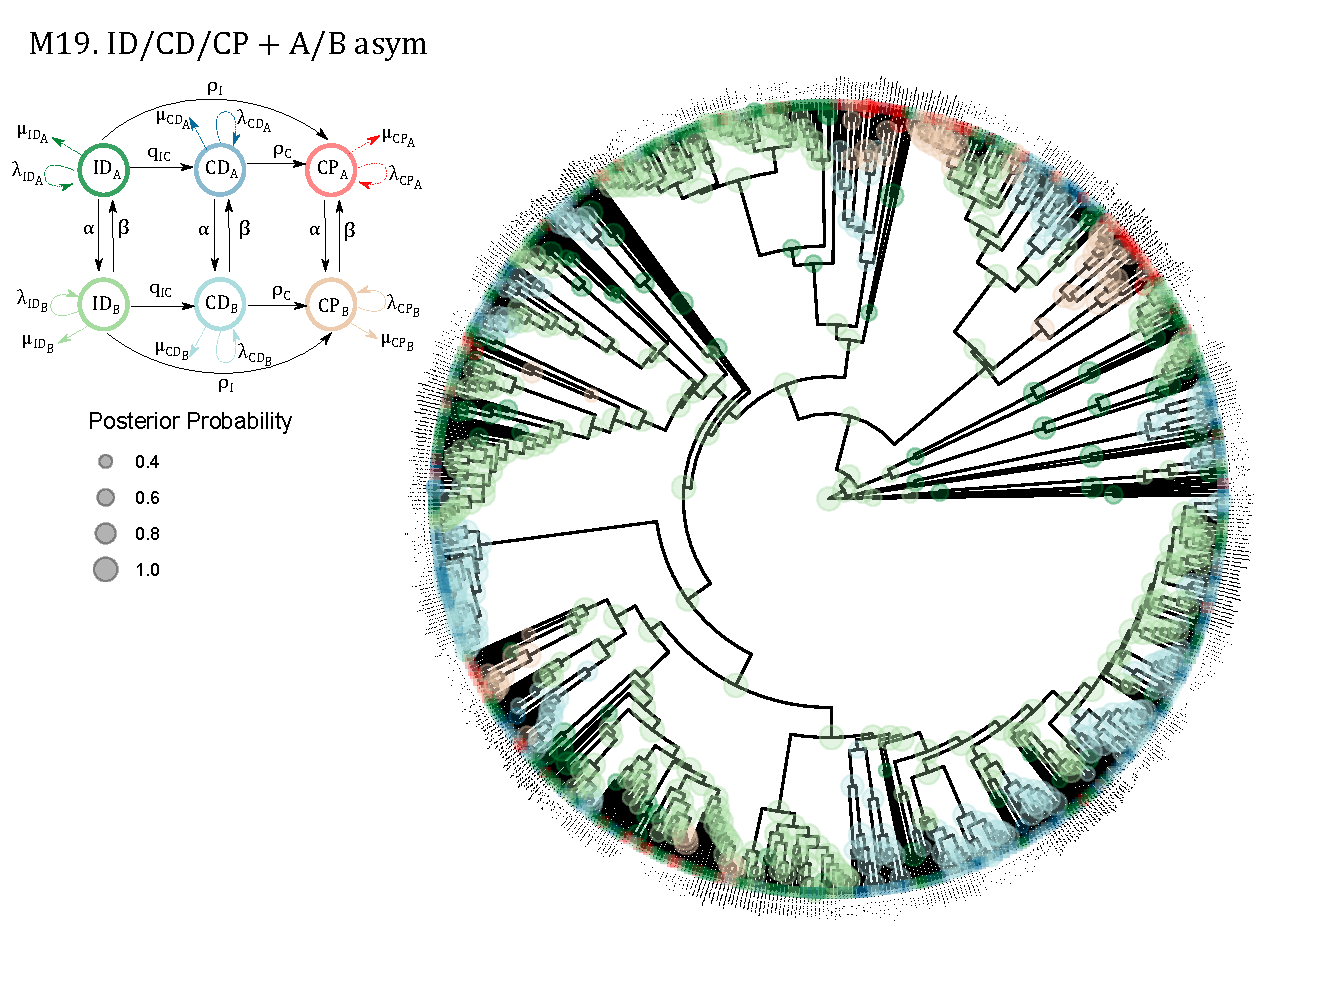
\includegraphics[width=\textwidth]{figS14.pdf}
\caption{Ancestral state estimation showing the maximum \emph{a posteriori} estimates of the marginal probability distributions for each of the 650 internal nodes under the  ploidy, breeding systems, and hidden states model (M19).} % XXX
\label{suppfigure:IDCDCPnodipABasr}
\end{suppfigure}



\begin{suppfigure}
%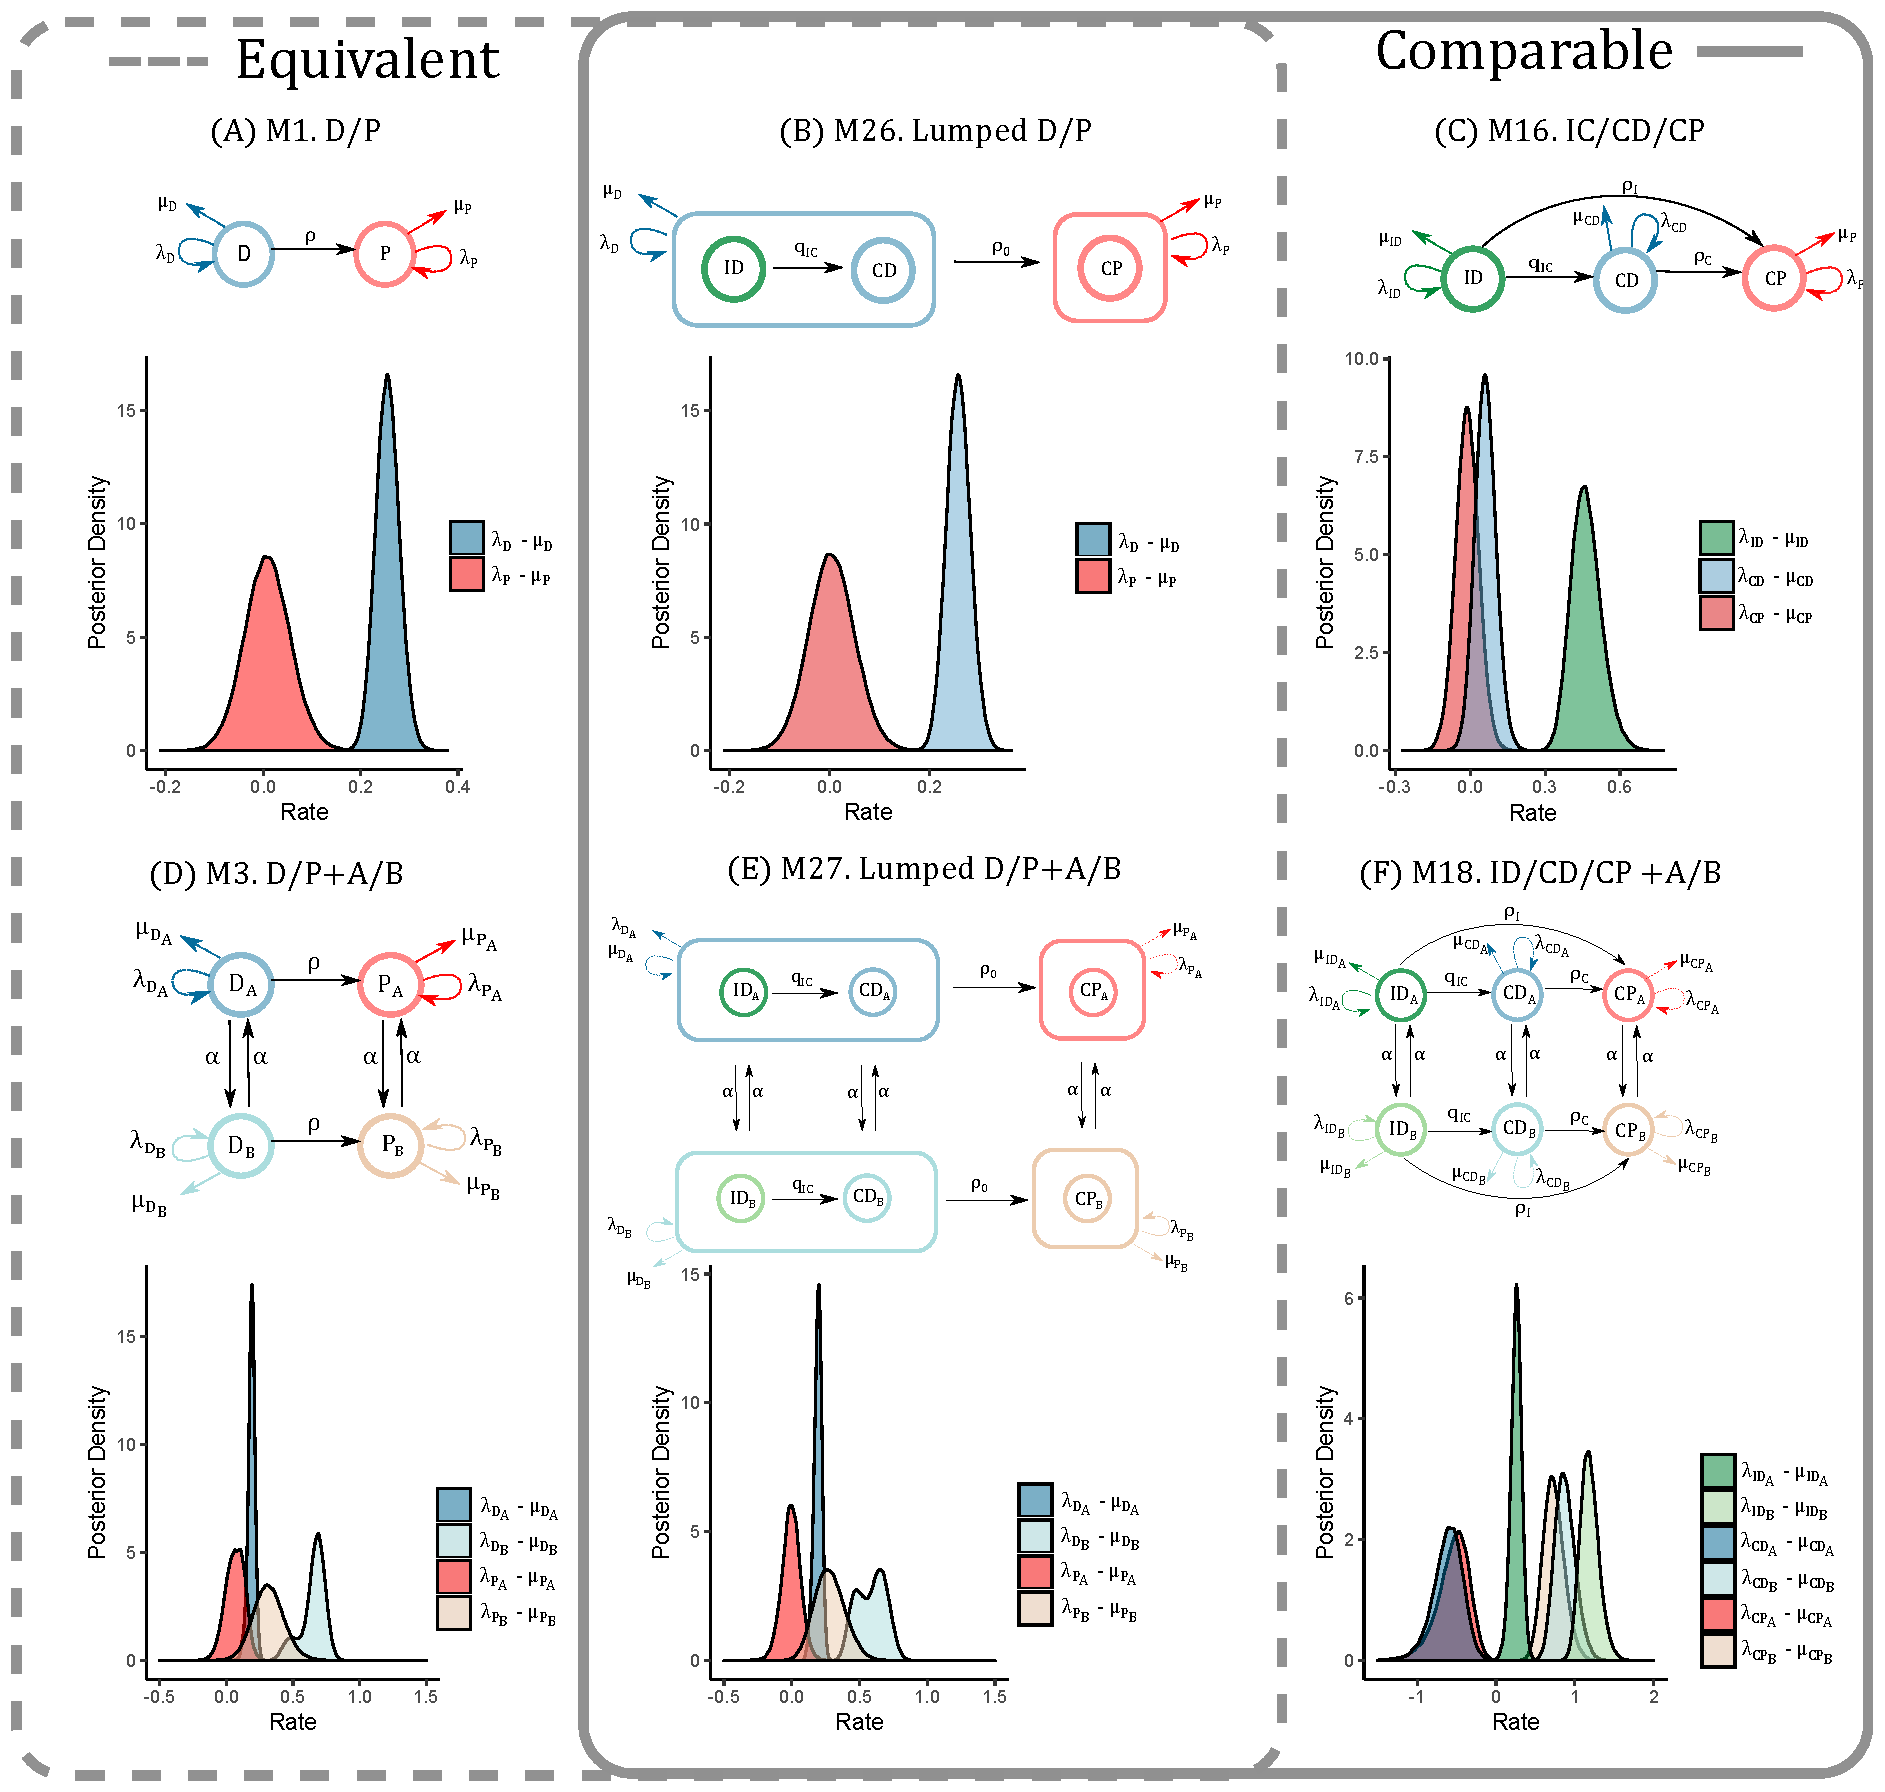
\includegraphics[width=\textwidth]{figS15.pdf}
\caption{Testing the addition of breeding system to ploidy models. (A) Ploidy only model (M1) where data enter as binary $D$ and $P$. (B) Lumped model for ploidy (M26) where data are the three-state values ($ID,CP,CD$) but results are equivalent to model M1.  (C) Ploidy and breeding system model (M16) where  data enter as the three-state values. Models M26 and M16 are comparable whereas M1 and M16 are not. (D) Ploidy and hidden state model (M3) where data enter as binary $D$ and $P$. (E) Lumped model for ploidy and hidden state (M27) where data are the three-state values ($ID,CP,CD$) but results are equivalent to model M3. (F) Ploidy, breeding system, and hidden state model (M18) where  data enter as the three-state values. Models M27 and M18 are comparable whereas M3 and M18 are not. Bayes factors comparing the models are shown in \cref{table:lumped}.} % XXX
\label{suppfigure:lumpedDP}
\end{suppfigure}

\begin{suppfigure}
%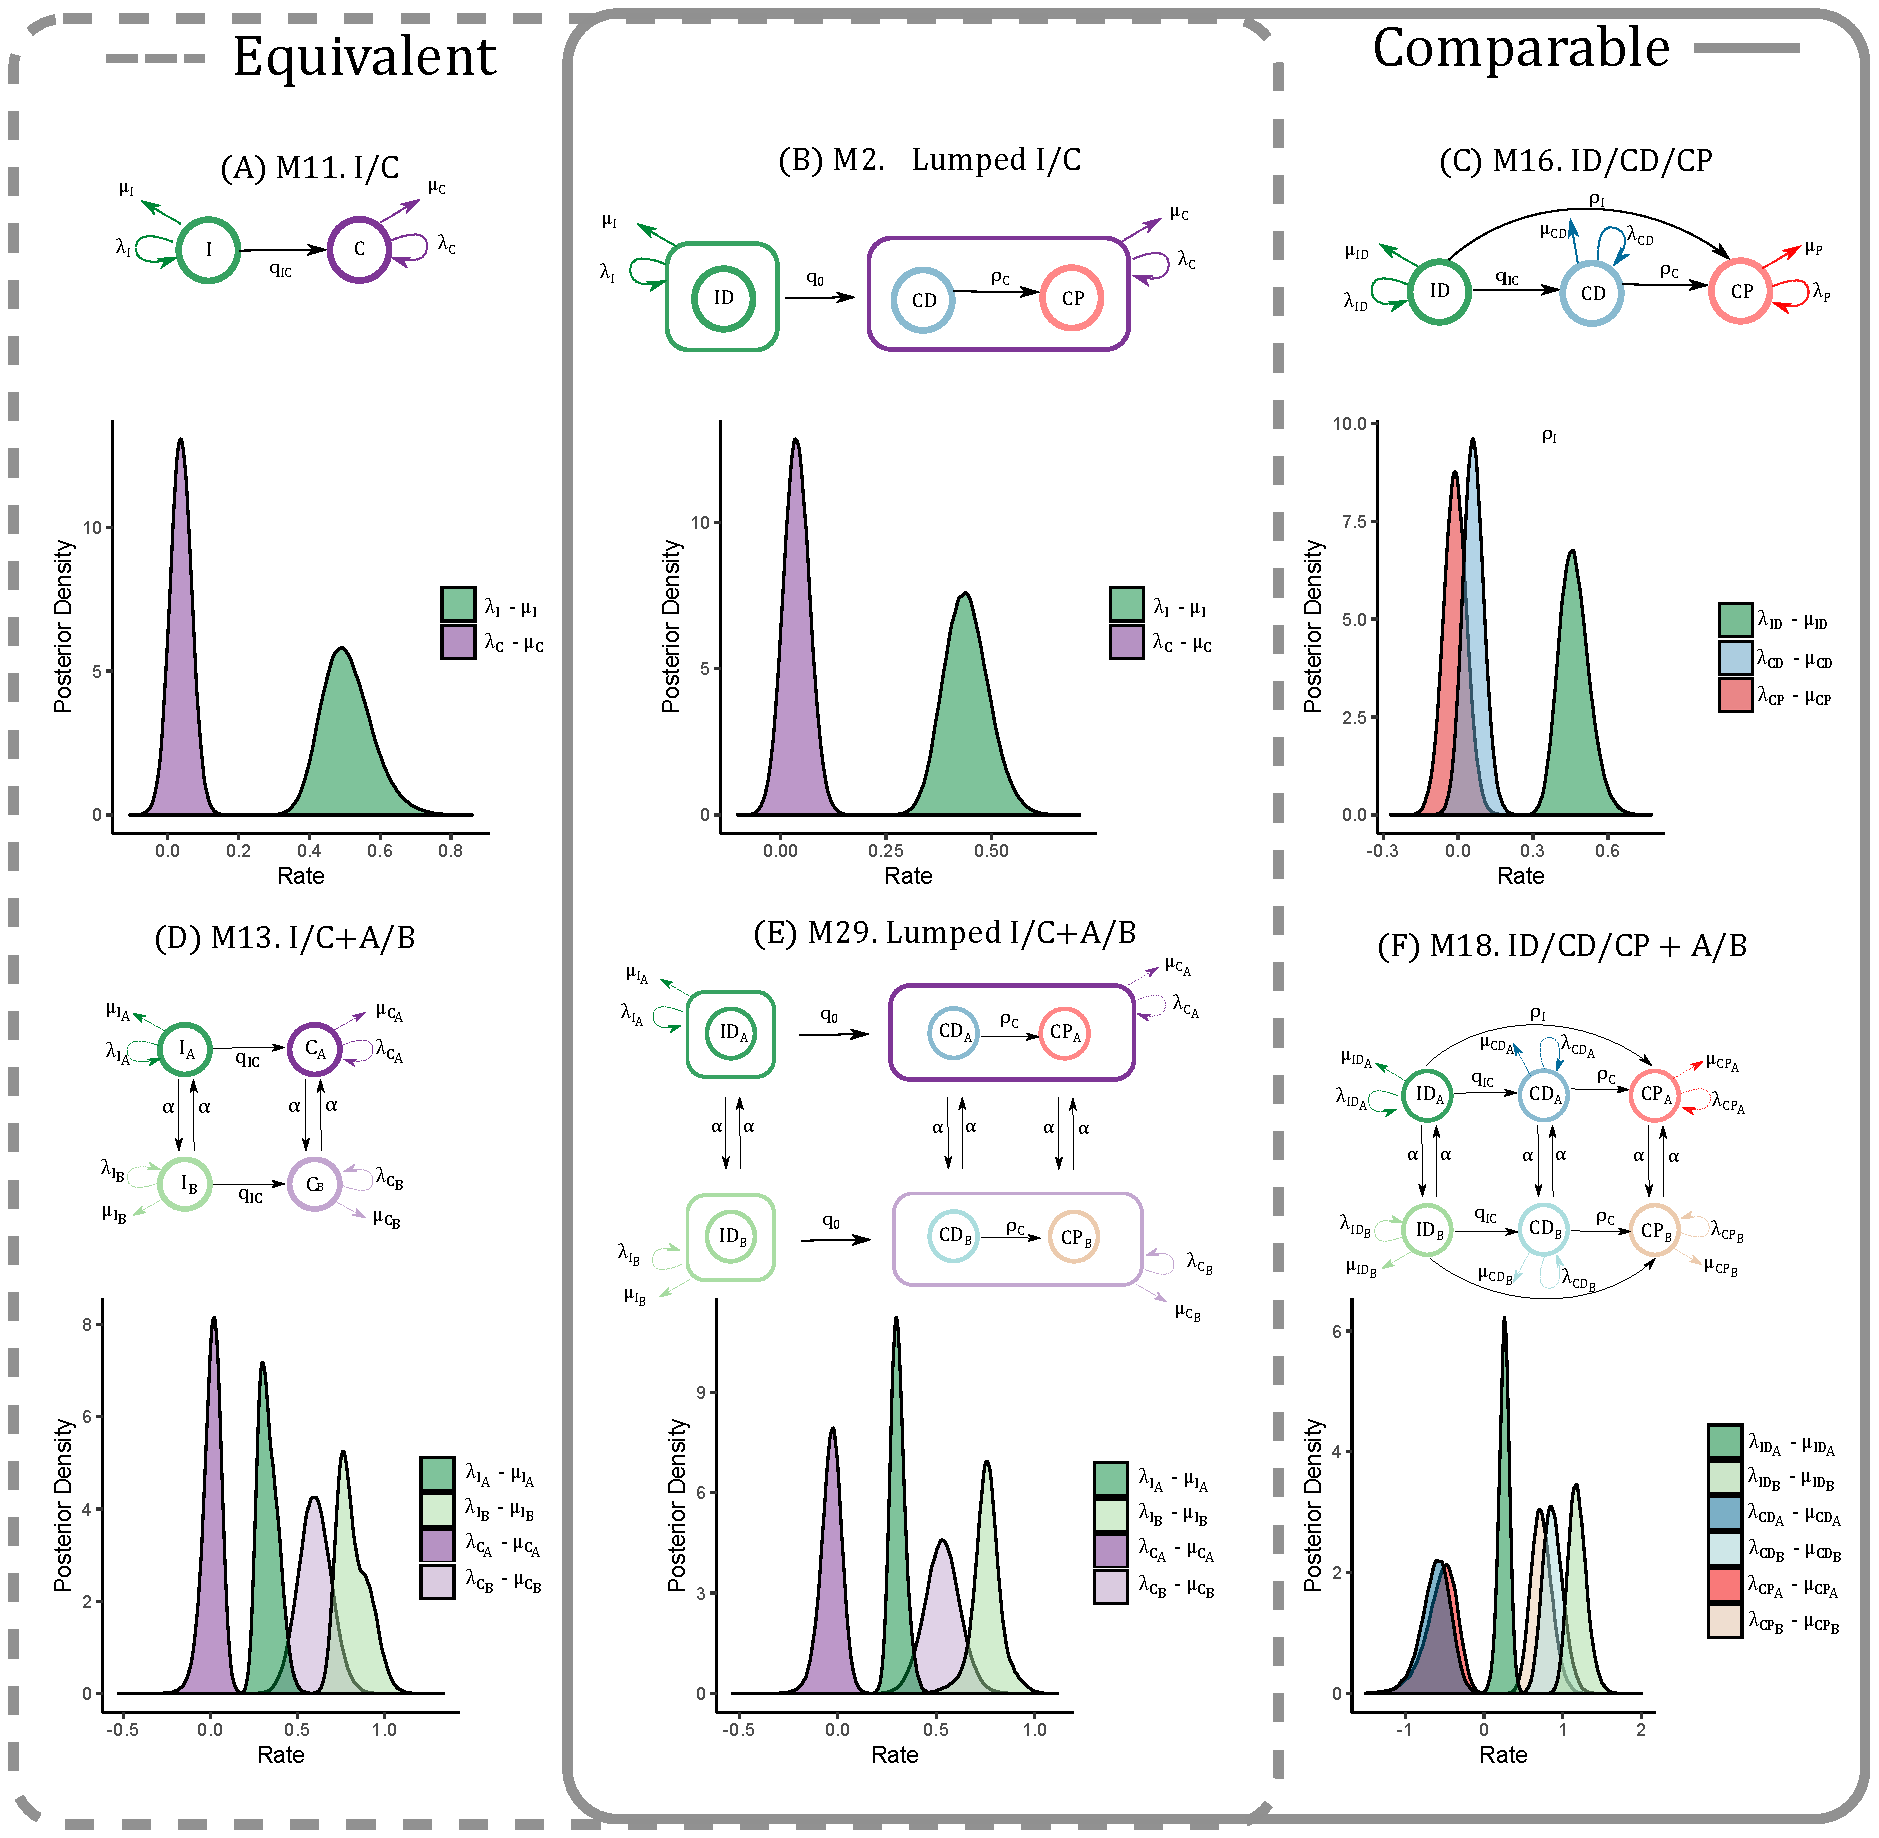
\includegraphics[width=\textwidth]{figS16.pdf}
\caption{Testing the addition of ploidy to breeding system models. (A) Breeding system only model (M11) where data enter as binary $I$ and $C$. (B) Lumped model for breeding system (M28) where data are the three-state values ($ID,CP,CD$) but results are equivalent to model M11.  (C) Ploidy and breeding system model (M16) where  data enter as the three-state values. Models M28 and M16 are comparable whereas M11 and M16 are not. (D) Breeding system and hidden state model (M13) where data enter as binary $I$ and $C$. (E) Lumped model for breeding system and hidden state (M29) where data are the three-state values ($ID,CP,CD$) but results are equivalent to model M13. (F) Ploidy, breeding system, and hidden state model (M18) where  data enter as the three-state values. Models M29 and M18 are comparable whereas M13 and M18 are not. Bayes factors comparing the models are shown in \cref{table:lumped}.} % XXX
\label{suppfigure:lumpedIC}
\end{suppfigure}


\begin{suppfigure}
%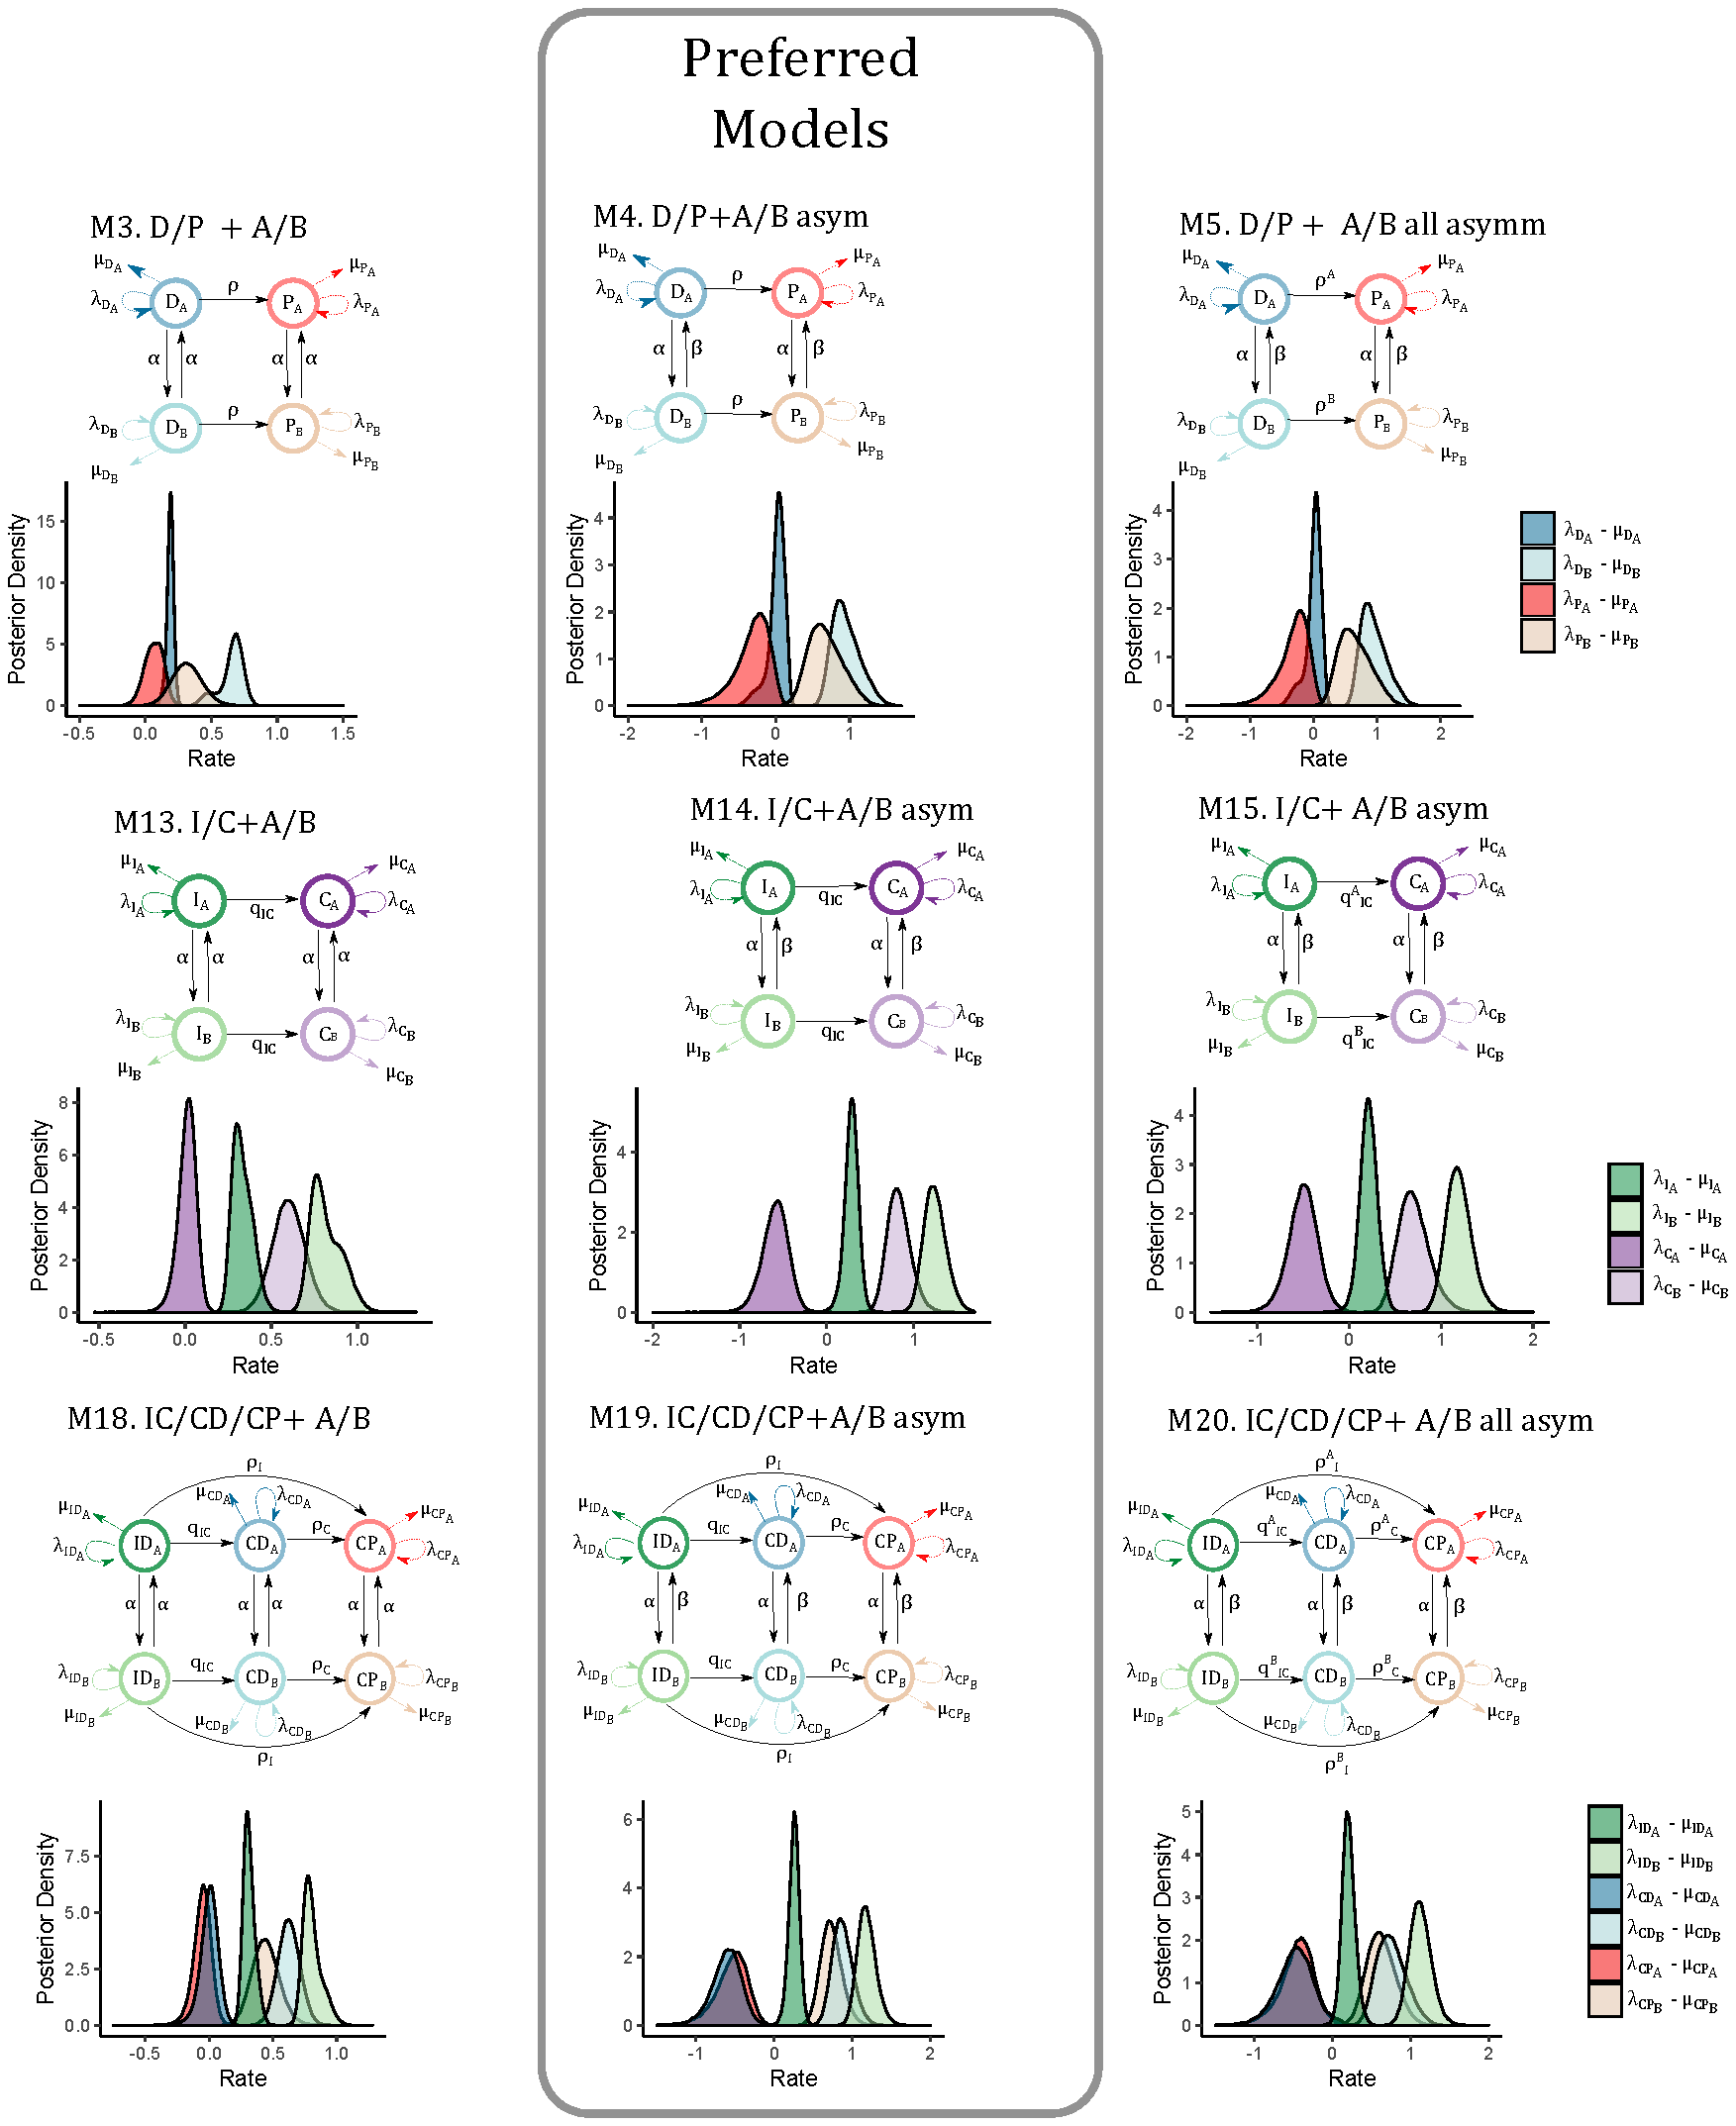
\includegraphics[width=\textwidth]{figS17.pdf}
\caption{Effect of asymmetric rates in hidden models. First column models M3, M13, and M18 assume that the rates between hidden states are equal. The models in the second column (M4, M14, M19) assume that the rates between hidden states are different . Column three models assumes that the rates between hidden state are asymmetric and that the transition rates within each hidden states are also different. Bayes factors in \cref{supptable:asymmetry} strongly preferred models with asymmetric rates between states (second column) over models with equal rates in hidden states (first column). Models in the second column are moderately or equally prefer to more complex models in column 3. } % XXX
\label{suppfigure:asymmetric}
\end{suppfigure}

\begin{suppfigure}
%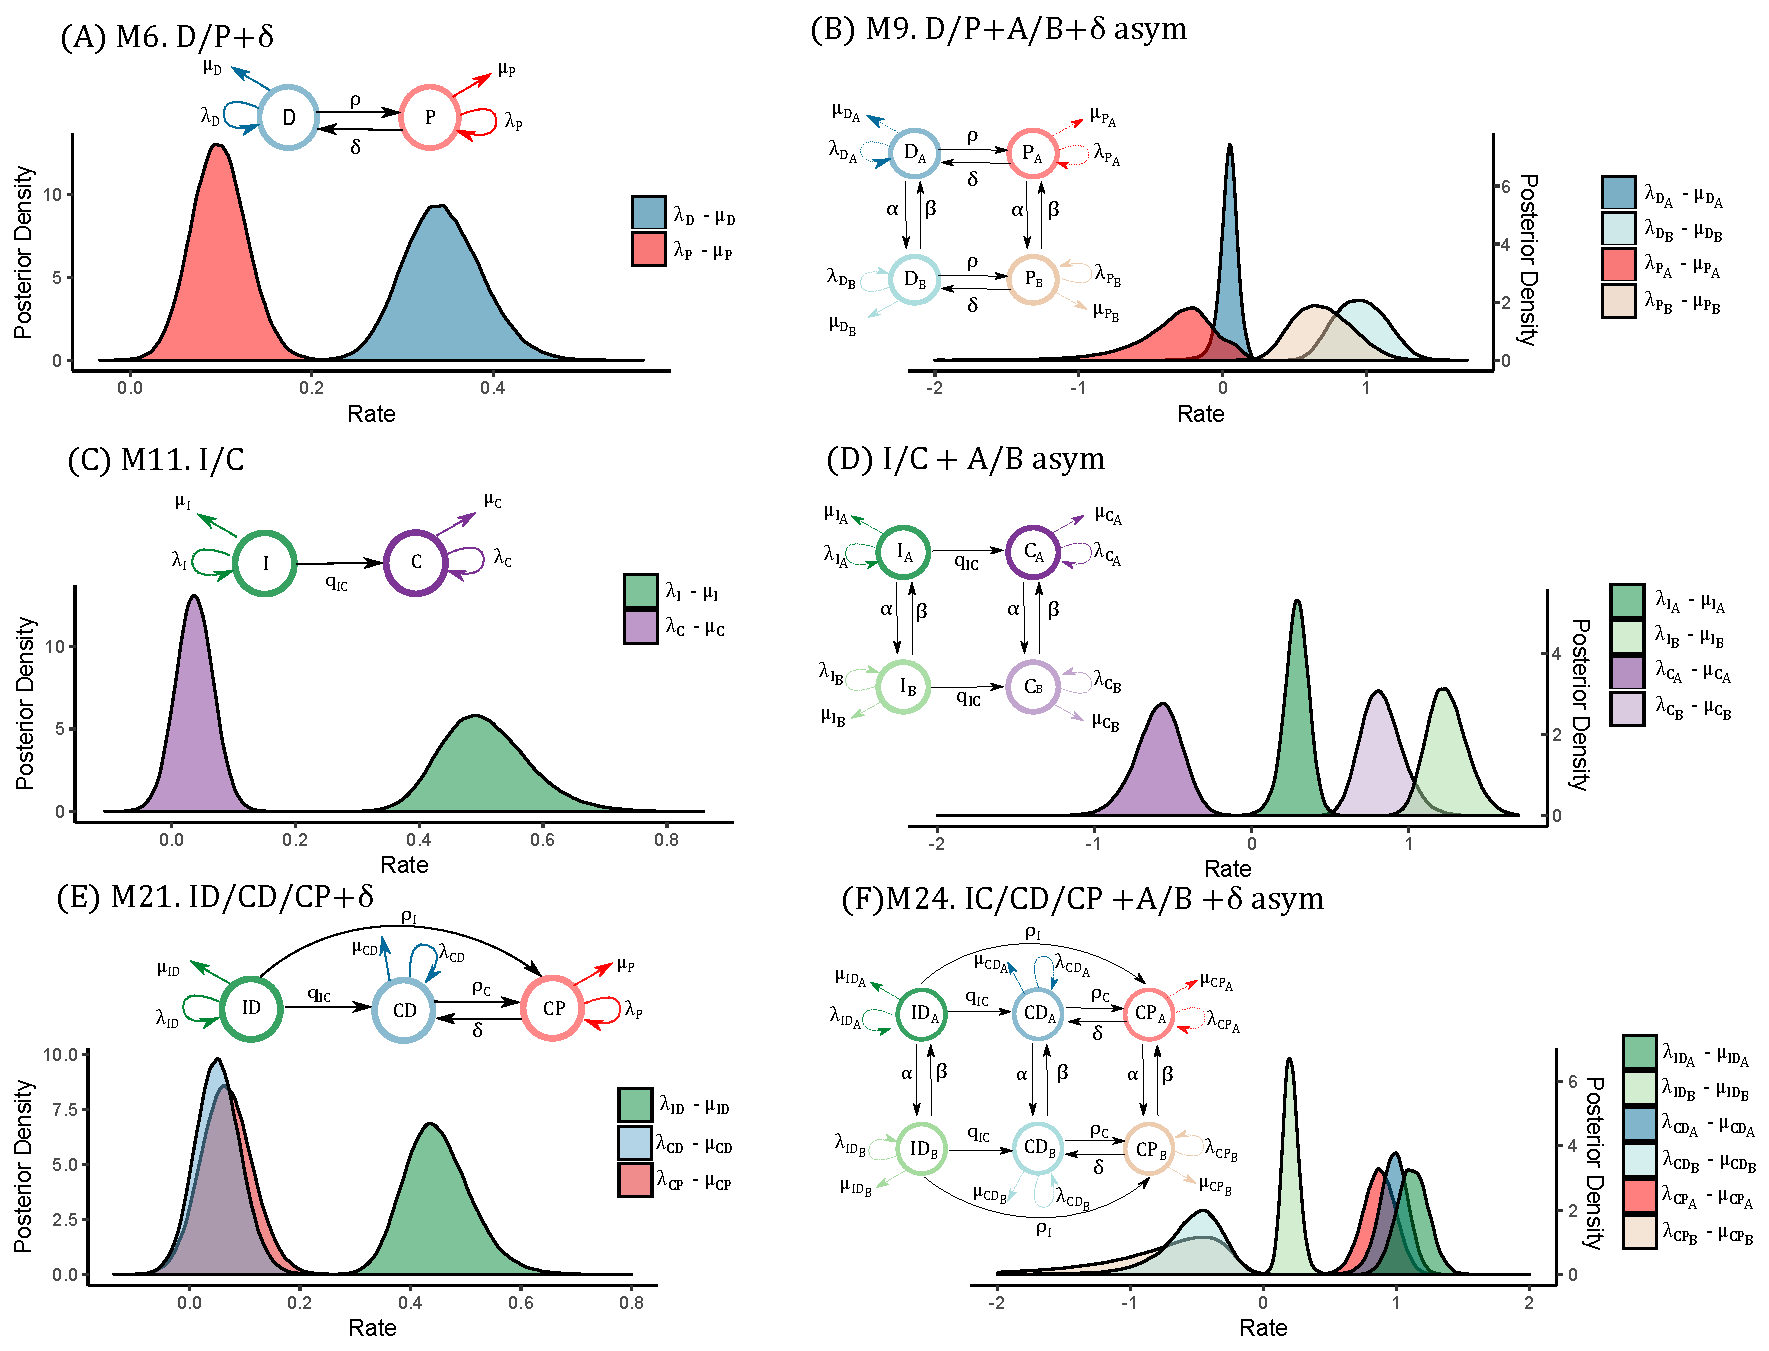
\includegraphics[width=\textwidth]{figS18.pdf}
\caption{Posterior distributions for the net diversification rates of the preferred models with diploidization. Red color represents diploid state $D$, blue color represents polyploid state $P$, green color represents self-incompatible $I$, purple color represents self-compatible $C$,  dark colors represent hidden state $A$ and light colors hidden state $B$.  (A) Ploidy only model M6. (B) Ploidy and hidden states model M9 (C) Breeding systems only model M11. (D) Breeding systems and hidden state model M14. (E) Ploidy and breeding systems model M21. (F) Ploidy, breeding systems, and hidden states model M24.} % XXX
\label{suppfigure:alldip}
\end{suppfigure}

% Supplementary TABLES

\begin{supptable}
\addtolength{\tabcolsep}{-3pt}
\begin{tabular}{|l|r|c|c|c|c|l|}
\hline
Model                           & \begin{tabular}[c]{@{}l@{}}Marginal\\ log-likelihood\end{tabular} & M7    & M8     & M9    & M10   & Evidence                                                                                     \\ \hline
M6. D/P+$\delta$                & -1268.83                                                          & 55.41 & 42.78  & 53.37 & 52.85 & \begin{tabular}[c]{@{}l@{}}Every model strongly \\ preferred over M6\end{tabular}            \\ \hline
\textbf{M7. CID D/P+$\delta$}   & \textbf{-1212.42}                                                 &       & -12.62 & -2.04 & -2.04 & \begin{tabular}[c]{@{}l@{}}Model M7 moderately\\ preferred over M9 and M10\end{tabular}      \\ \hline
M8. D/P+A/B $\delta$            & -1214.46                                                          &       &        & 10.58 & 10.07 & \begin{tabular}[c]{@{}l@{}}Asymmetric rates strongly\\ preferred over symmetric\end{tabular} \\ \hline
M9. D/P+A/B +$\delta$ asym      & -1214.46                                                          &       &        &       & -0.51 & No evidence                                                                                  \\ \hline
M10. D/P+A/B +$\delta$ all asym & -1214.97                                                          &       &        &       &       &         \\ \hline                                                                                    
\end{tabular}
\caption{Bayes factors in log-scale of  ploidy only models with diplodization. Results indicate that a character independent model (M7) is strongly preferred over model M6 (BiSSE). Model M7 (bold) is also moderately preferred over any of the HiSSE models with asymmetric hidden rates (M9, M10).}
\label{supptable:M6M10}
\end{supptable}

\begin{supptable}
\addtolength{\tabcolsep}{-3pt}
\begin{tabular}{|l|r|c|c|c|c|l|}
\hline
Model                            & \begin{tabular}[c]{@{}l@{}}Marginal\\ log-likelihood\end{tabular} & M18   & M19   & M20   & Evidence                                                                                                   \\ \hline
M16. ID/CP/CD                    & -1459.11                                                          & 45.11 & 65.91 & 63.98 & \begin{tabular}[c]{@{}l@{}}Every model strongly \\ preferred over M16\end{tabular}                         \\ \hline
M17. CID ID/CP/CD                & *                                                                 &       &       &       &                                                                                                            \\
M18. ID/CP/CD+A/B                & -1414                                                             &       & 20.79 & 18.87 & \begin{tabular}[c]{@{}l@{}}Asymmetric rates strongly\\ preferred over symmetric\end{tabular}               \\ \hline
\textbf{M19. ID/CP/CD +A/B asym} & \textbf{-1393.20}                                                 &       &       & -1.92 & \begin{tabular}[c]{@{}l@{}}Asymmetric hidden rates moderately\\ preferred over all asymmetric\end{tabular} \\ \hline
M20. ID/CP/CD +A/B all asym      & -1393.12                                                          &       &       &       &   \\ \hline                                                                                                        
\end{tabular}
\caption{Bayes factors of ploidy and breeding system without diploidization in log-scale. Results indicate that the model with asymmetric hidden rates (M19, bold) is  strongly preferred over M16 and M18 and moderately preferred over the MuHiSSe with all rates asymetric (M20). *Marginal log-likelihood for M17 could not be calculated within allotted computer time.}
\label{supptable:M16M20}
\end{supptable}

\begin{supptable}
\addtolength{\tabcolsep}{-3pt}
\begin{tabular}{|l|r|c|c|c|c|l|}
\hline
Model                                 & \begin{tabular}[c]{@{}l@{}}Marginal\\ log-likelihood\end{tabular} & M22   & M23    & M24   & M25   & Evidence                                                                                         \\ \hline
M21. ID/CP/CD+$\delta$                & -1454.68                                                          & 55.48 & 46.031 & 67.94 & 65.15 & \begin{tabular}[c]{@{}l@{}}Every model strongly \\ preferred over M21\end{tabular}               \\ \hline
M22. CID ID/CP/CD+$\delta$            & -1399.201                                                         &       & -9.452 & 12.45 & 9.675 & \begin{tabular}[c]{@{}l@{}}Model M24 strongly preferred \\ over M22\end{tabular}                 \\ \hline
M23. ID/CP/CD+A/B $\delta$            & -1408.65                                                          &       &        & 21.91 & 19.12 & \begin{tabular}[c]{@{}l@{}}Asymmetric rates strongly\\ preferred over symmetric\end{tabular}     \\ \hline
\textbf{M24. ID/CP/CD +$\delta$ asym} & \textbf{-1386.74}                                                 &       &        &       & -2.78 & \begin{tabular}[c]{@{}l@{}}Asymmetric hidden rates \\ preferred over all asymmetric\end{tabular} \\ \hline
M25. ID/CP/CD +$\delta$ all asym      & -1389.52                                                          &       &        &       &       &                      \\ \hline                                                                           
\end{tabular}
\caption{Bayes factors of ploidy and breeding system with diploidization in log-scale. Results indicate that the MuHiSSE model with asymmetric hidden rates (M24, bold) is  strongly preferred over M21-M23 and moderately preferred over the MuHiSSe with all rates asymmetric (M25).}
\label{supptable:M21M25}
\end{supptable}

\begin{supptable}
\addtolength{\tabcolsep}{-5pt}
\begin{tabular}{|l|c|c|c|c|}
\hline
Model                                    & \begin{tabular}[c]{@{}l@{}}Marginal\\ log-likelihood\end{tabular} & Comparison  & K=log(BF(M1,M2) & \begin{tabular}[c]{@{}l@{}}Preferred\\ Model (Evidence)\end{tabular} \\ \hline
M1. D/P                                  & -1238.76                                                          & M1 vs. M4   & 60.47           & M4 (Strong)                                                          \\
\textbf{M4. D/P+A/B asym}                & \textbf{-1223.28}                                                &             &                 &                                                                      \\ \hline
M11. I/C                                 & -1309.07                                                          & M11 vs. M14 & 61.35           & M14 (Strong)                                                         \\
\textbf{M14. I/C+A/B asym}               & \textbf{-1247.72}                                                 &             &                 &                                                                      \\ \hline
M16. ID/CD/CP                            & -1459.11                                                          & M16 vs. M19 & 65.90           & M19 (Strong)                                                         \\
\textbf{M19. ID/CD/CP+A/B asym}          & \textbf{-1393.20}                                                &             &                 &                                                                      \\ \hline
M6. D/P+$\delta$                         & -1283.76                                                          & M6 vs. M9   & 69.3            & M9 (Strong)                                                          \\
\textbf{M9. D/P+A/B+$\delta$ asym}       & \textbf{-1214.46}                                                 &             &                 &                                                                      \\ \hline
M21. IC/CD/CP+$\delta$                   & -1454.68                                                          & M21 vs. M24 & 68.48           & M24 (Strong)                                                         \\
\textbf{M24. IC/CD/CP+A/B+$\delta$ asym} & \textbf{-1386.20}                                                 &             &                 &                                                                      \\ \hline
\end{tabular}
\caption{Test for addition of hidden states in models via Bayes factors (in log-scale). Models with hidden states  (M4, M14, M19, M9, M24, bold) are strongly preferred over simpler models that do not include hidden s}
\label{supptable:testaddhidden}
\end{supptable}


\begin{supptable}
\addtolength{\tabcolsep}{-5pt}
\begin{tabular}{|l|c|c|c|l|}
\hline
Model                                    & \begin{tabular}[c]{@{}l@{}}Marginal\\ log-likelihood\end{tabular} & Comparison  & K=log(BF(M1,M2) & \begin{tabular}[c]{@{}l@{}}Preferred\\ Model (Evidence)\end{tabular} \\ \hline
M3. D/P+A/B                                 & -1234.52                     &    M3 vs. M4                 & 11.239                  & M4 (Strong)   \\
\textbf{M4. D/P+ A/B asym}            & -1223.28                     &   M4 vs. M5              & -1.658                  & M4 (Moderate)   \\
M5. D/P+A/B all asym                 & -1224.93                     &                     &                         &                         \\ \hline
M13. I/C+ A/B                                & -1270.47                     &   M13 vs. M14                  & 22.75                   & M14 (Strong)   \\
\textbf{M14. I/C+ A/B asym}            & \textbf{-1247.72}            & M14 vs. M15         & {0.05}           & No evidence             \\
M15. I/C+ A/B all asym               & -1247.67                     &                     &                         &                         \\ \hline
M18. IC/CD/CP+A/B                            & -1414.00                     &     M18 vs. M19                & 20.79                   & M19 (Strong)    \\
\textbf{M19. IC/CD/CP+ A/B asym}       & \textbf{-1393.21}            & M19 vs. M20          & {-1.919}         & M19 (Moderate)   \\
M20. IC/CD/CP+ A/B all asym           & -1395.129                    &                     &                         &                         \\ \hline
M8. D/P +A/B+$\delta$                          & -1225.05                     &  M8 vs. M9                   & 10.58                   & M9 (Strong)    \\
\textbf{M9. D/P+ A/B+ $\delta$ asym}      & \textbf{-1214.46}                     &    M9 vs. M10                 & -0.52                   & M10 (Moderate) \\
M10. D/P+A/B+$\delta$ all asym        & -1214.98                     &                    &                         &                         \\ \hline
M23. IC/CD/DP+A/B+$\delta$                 & -1408.65                     &     M23 vs M24                & 21.91                   & M24(Strong)     \\
\textbf{M24. IC/CD/DP+A/B+$\delta$ asym} & \textbf{-1386.74}                     &   M24 vs M25              & -2.78                   & M24 (Moderate) \\
M25. IC/CD/DP+A/B+ $\delta$ all asym     & -1389.52                     &                     &                         &                         \\ \hline
\end{tabular}
\caption{Test for asymmetry of the hidden trait transition rates via Bayes factors. For all models, asymmetric transition rates between hidden trait states are preferred over models with equal rates (bold). Adding more complexity by assuming asymmetry in all rates within both hidden states is not preferred over models with just asymmetry between hidden states.} 
\label{supptable:asymmetry}
\end{supptable}


\begin{supptable}
\addtolength{\tabcolsep}{-3pt}
\begin{tabular}{|l|c|c|c|c|}
\hline
Model                                    & \begin{tabular}[c]{@{}l@{}}Marginal\\ log-likelihood\end{tabular} & Comparison  & K=log(BF(M1,M2) & \begin{tabular}[c]{@{}l@{}}Preferred\\ Model (Evidence)\end{tabular} \\ \hline
M1. D/P                                  & -1238.76                                                          & M1 vs. M6   & 65.92           & M6 (Strong)                                                          \\
\textbf{M6. D/P+$\delta$}                & \textbf{-1267.84}                                                 &             &                 &                                                                      \\ \hline
M4. D/P+A/B asym                         & -1223.28                                                          & M4 vs. M9   & 8.81            & M9 (Moderate)                                                        \\
\textbf{M9. D/P+A/B+$\delta$ asym}       & \textbf{-1214.46}                                                 &             &                 &                                                                      \\ \hline
M16. ID/CD/CP                            & -1459.11                                                          & M16 vs. M21 & 4.41            & M21 (Moderate)                                                       \\
\textbf{M21. ID/CD/CP+$\delta$}          & \textbf{-1454.68}                                                 &             &                 &                                                                      \\ \hline
M19. IC/CD/CP +A/B asym                       & -1393.20                                                          & M19 vs. M24 & 6.46            & M24 (Moderate)                                                       \\
\textbf{M24. IC/CD/CP+A/B+$\delta$ asym} & \textbf{-1386.20}                                                 &             &                 &                                                                      \\ \hline
\end{tabular}
\caption{Test for inclusion of a diploidization rate via Bayes factors. Models with diploidization are moderately preferred over models that do not include a diploidization rate (bold).}
\label{supptable:testdiploidization}
\end{supptable}



